% Options for packages loaded elsewhere
\PassOptionsToPackage{unicode}{hyperref}
\PassOptionsToPackage{hyphens}{url}
%
\documentclass[
]{article}
\usepackage{amsmath,amssymb}
\usepackage{lmodern}
\usepackage{iftex}
\ifPDFTeX
  \usepackage[T1]{fontenc}
  \usepackage[utf8]{inputenc}
  \usepackage{textcomp} % provide euro and other symbols
\else % if luatex or xetex
  \usepackage{unicode-math}
  \defaultfontfeatures{Scale=MatchLowercase}
  \defaultfontfeatures[\rmfamily]{Ligatures=TeX,Scale=1}
\fi
% Use upquote if available, for straight quotes in verbatim environments
\IfFileExists{upquote.sty}{\usepackage{upquote}}{}
\IfFileExists{microtype.sty}{% use microtype if available
  \usepackage[]{microtype}
  \UseMicrotypeSet[protrusion]{basicmath} % disable protrusion for tt fonts
}{}
\makeatletter
\@ifundefined{KOMAClassName}{% if non-KOMA class
  \IfFileExists{parskip.sty}{%
    \usepackage{parskip}
  }{% else
    \setlength{\parindent}{0pt}
    \setlength{\parskip}{6pt plus 2pt minus 1pt}}
}{% if KOMA class
  \KOMAoptions{parskip=half}}
\makeatother
\usepackage{xcolor}
\usepackage[margin=1in]{geometry}
\usepackage{color}
\usepackage{fancyvrb}
\newcommand{\VerbBar}{|}
\newcommand{\VERB}{\Verb[commandchars=\\\{\}]}
\DefineVerbatimEnvironment{Highlighting}{Verbatim}{commandchars=\\\{\}}
% Add ',fontsize=\small' for more characters per line
\usepackage{framed}
\definecolor{shadecolor}{RGB}{248,248,248}
\newenvironment{Shaded}{\begin{snugshade}}{\end{snugshade}}
\newcommand{\AlertTok}[1]{\textcolor[rgb]{0.94,0.16,0.16}{#1}}
\newcommand{\AnnotationTok}[1]{\textcolor[rgb]{0.56,0.35,0.01}{\textbf{\textit{#1}}}}
\newcommand{\AttributeTok}[1]{\textcolor[rgb]{0.77,0.63,0.00}{#1}}
\newcommand{\BaseNTok}[1]{\textcolor[rgb]{0.00,0.00,0.81}{#1}}
\newcommand{\BuiltInTok}[1]{#1}
\newcommand{\CharTok}[1]{\textcolor[rgb]{0.31,0.60,0.02}{#1}}
\newcommand{\CommentTok}[1]{\textcolor[rgb]{0.56,0.35,0.01}{\textit{#1}}}
\newcommand{\CommentVarTok}[1]{\textcolor[rgb]{0.56,0.35,0.01}{\textbf{\textit{#1}}}}
\newcommand{\ConstantTok}[1]{\textcolor[rgb]{0.00,0.00,0.00}{#1}}
\newcommand{\ControlFlowTok}[1]{\textcolor[rgb]{0.13,0.29,0.53}{\textbf{#1}}}
\newcommand{\DataTypeTok}[1]{\textcolor[rgb]{0.13,0.29,0.53}{#1}}
\newcommand{\DecValTok}[1]{\textcolor[rgb]{0.00,0.00,0.81}{#1}}
\newcommand{\DocumentationTok}[1]{\textcolor[rgb]{0.56,0.35,0.01}{\textbf{\textit{#1}}}}
\newcommand{\ErrorTok}[1]{\textcolor[rgb]{0.64,0.00,0.00}{\textbf{#1}}}
\newcommand{\ExtensionTok}[1]{#1}
\newcommand{\FloatTok}[1]{\textcolor[rgb]{0.00,0.00,0.81}{#1}}
\newcommand{\FunctionTok}[1]{\textcolor[rgb]{0.00,0.00,0.00}{#1}}
\newcommand{\ImportTok}[1]{#1}
\newcommand{\InformationTok}[1]{\textcolor[rgb]{0.56,0.35,0.01}{\textbf{\textit{#1}}}}
\newcommand{\KeywordTok}[1]{\textcolor[rgb]{0.13,0.29,0.53}{\textbf{#1}}}
\newcommand{\NormalTok}[1]{#1}
\newcommand{\OperatorTok}[1]{\textcolor[rgb]{0.81,0.36,0.00}{\textbf{#1}}}
\newcommand{\OtherTok}[1]{\textcolor[rgb]{0.56,0.35,0.01}{#1}}
\newcommand{\PreprocessorTok}[1]{\textcolor[rgb]{0.56,0.35,0.01}{\textit{#1}}}
\newcommand{\RegionMarkerTok}[1]{#1}
\newcommand{\SpecialCharTok}[1]{\textcolor[rgb]{0.00,0.00,0.00}{#1}}
\newcommand{\SpecialStringTok}[1]{\textcolor[rgb]{0.31,0.60,0.02}{#1}}
\newcommand{\StringTok}[1]{\textcolor[rgb]{0.31,0.60,0.02}{#1}}
\newcommand{\VariableTok}[1]{\textcolor[rgb]{0.00,0.00,0.00}{#1}}
\newcommand{\VerbatimStringTok}[1]{\textcolor[rgb]{0.31,0.60,0.02}{#1}}
\newcommand{\WarningTok}[1]{\textcolor[rgb]{0.56,0.35,0.01}{\textbf{\textit{#1}}}}
\usepackage{graphicx}
\makeatletter
\def\maxwidth{\ifdim\Gin@nat@width>\linewidth\linewidth\else\Gin@nat@width\fi}
\def\maxheight{\ifdim\Gin@nat@height>\textheight\textheight\else\Gin@nat@height\fi}
\makeatother
% Scale images if necessary, so that they will not overflow the page
% margins by default, and it is still possible to overwrite the defaults
% using explicit options in \includegraphics[width, height, ...]{}
\setkeys{Gin}{width=\maxwidth,height=\maxheight,keepaspectratio}
% Set default figure placement to htbp
\makeatletter
\def\fps@figure{htbp}
\makeatother
\setlength{\emergencystretch}{3em} % prevent overfull lines
\providecommand{\tightlist}{%
  \setlength{\itemsep}{0pt}\setlength{\parskip}{0pt}}
\setcounter{secnumdepth}{5}
\ifLuaTeX
  \usepackage{selnolig}  % disable illegal ligatures
\fi
\IfFileExists{bookmark.sty}{\usepackage{bookmark}}{\usepackage{hyperref}}
\IfFileExists{xurl.sty}{\usepackage{xurl}}{} % add URL line breaks if available
\urlstyle{same} % disable monospaced font for URLs
\hypersetup{
  pdftitle={QALL401: Data Analysis for Researchers},
  hidelinks,
  pdfcreator={LaTeX via pandoc}}

\title{QALL401: Data Analysis for Researchers}
\author{}
\date{\vspace{-2.5em}}

\begin{document}
\maketitle

\hypertarget{course-contents}{%
\subsection*{Course Contents}\label{course-contents}}
\addcontentsline{toc}{subsection}{Course Contents}

\begin{enumerate}
\def\labelenumi{\arabic{enumi}.}
\tightlist
\item
  2022.12.07: Introduction: About the course {[}lead by TK{]}

  \begin{itemize}
  \tightlist
  \item
    An introduction to open and public data, and data science
  \end{itemize}
\item
  2022-12-14: Exploratory Data Analysis (EDA) 1 {[}lead by hs{]}

  \begin{itemize}
  \tightlist
  \item
    R Basics with RStudio and/or RStudio.cloud; Toy Data
  \end{itemize}
\item
  2022-12-21: Exploratory Data Analysis (EDA) 2 {[}lead by hs{]}

  \begin{itemize}
  \tightlist
  \item
    R Markdown, \texttt{tidyverse} I: \texttt{dplyr}; \texttt{gapminder}
  \end{itemize}
\item
  2023-01-11: Exploratory Data Analysis (EDA) 3 {[}lead by hs{]}

  \begin{itemize}
  \tightlist
  \item
    \texttt{tidyverse}II: \texttt{readr}, \texttt{ggplot2}; Public Data,
    WDI, WIR, etc
  \end{itemize}
\item
  2023-01-18: Exploratory Data Analysis (EDA) 4 {[}lead by hs{]}

  \begin{itemize}
  \tightlist
  \item
    \texttt{tidyverse} III: \texttt{tidyr}, etc.; WDI, WIR, etc
  \end{itemize}
\item
  \textbf{2023-01-25: Exploratory Data Analysis (EDA) 5 {[}lead by hs{]}
  }

  \begin{itemize}
  \tightlist
  \item
    \texttt{tidyverse} IV; WDI, WIR, etc
  \end{itemize}
\item
  2023-02-01: Introduction to PPDAC

  \begin{itemize}
  \tightlist
  \item
    Problem-Plan-Data-Analysis-Conclusion Cycle: {[}lead by TK{]}
  \end{itemize}
\item
  2023-02-08: Model building I {[}lead by TK{]}

  \begin{itemize}
  \tightlist
  \item
    Collecting and visualizing data and Introduction to WDI\\
    (World Development Indicators by World Bank)
  \end{itemize}
\item
  2023-02-15: Model building II {[}lead by TK{]}

  \begin{itemize}
  \tightlist
  \item
    Analyzing data and communications
  \end{itemize}
\item
  2023-02-22: Project Presentation
\end{enumerate}

\hypertarget{exploratory-data-analysis-eda-i}{%
\section{Exploratory Data Analysis (EDA)
I}\label{exploratory-data-analysis-eda-i}}

\hypertarget{exploratory-data-analysis-ii}{%
\section{Exploratory Data Analysis
II}\label{exploratory-data-analysis-ii}}

\hypertarget{exploratory-data-analysis-iii}{%
\section{Exploratory Data Analysis
III}\label{exploratory-data-analysis-iii}}

\hypertarget{exploratory-data-analysis-eda-iv}{%
\section{Exploratory Data Analysis (EDA)
IV}\label{exploratory-data-analysis-eda-iv}}

\hypertarget{exploratory-data-analysis-eda-v}{%
\section{Exploratory Data Analysis (EDA)
V}\label{exploratory-data-analysis-eda-v}}

\begin{center}\rule{0.5\linewidth}{0.5pt}\end{center}

\hypertarget{setup}{%
\subsubsection*{Setup}\label{setup}}
\addcontentsline{toc}{subsubsection}{Setup}

\begin{Shaded}
\begin{Highlighting}[]
\FunctionTok{library}\NormalTok{(tidyverse)}
\end{Highlighting}
\end{Shaded}

\begin{verbatim}
## -- Attaching packages --------------------------------------- tidyverse 1.3.2 --
## v ggplot2 3.4.0      v purrr   1.0.0 
## v tibble  3.1.8      v dplyr   1.0.10
## v tidyr   1.2.1      v stringr 1.5.0 
## v readr   2.1.3      v forcats 0.5.2 
## -- Conflicts ------------------------------------------ tidyverse_conflicts() --
## x dplyr::filter() masks stats::filter()
## x dplyr::lag()    masks stats::lag()
\end{verbatim}

\begin{Shaded}
\begin{Highlighting}[]
\FunctionTok{library}\NormalTok{(WDI)}
\FunctionTok{library}\NormalTok{(readxl)}
\FunctionTok{library}\NormalTok{(broom)}
\end{Highlighting}
\end{Shaded}

\begin{itemize}
\tightlist
\item
  broom: \url{https://cran.r-project.org/web/packages/broom/index.html}
\item
  Introduction to broom:
  \url{https://cran.r-project.org/web/packages/broom/vignettes/broom.html}
\end{itemize}

\hypertarget{modeling}{%
\subsection{Modeling}\label{modeling}}

\hypertarget{what-is-modeling-in-eda}{%
\subsubsection{What is modeling in EDA}\label{what-is-modeling-in-eda}}

Model is a simple summary of data

Goal: A simple low-dimensional summary of a dataset. Ideally, the model
will capture true ``signals'' (i.e.~patterns generated by the phenomenon
of interest), and ignore ``noise'' (i.e.~random variation that you're
not interested in).

\begin{figure}
\centering
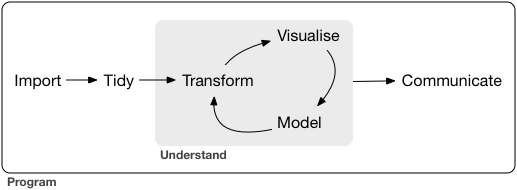
\includegraphics{data/data-science.png}
\caption{image}
\end{figure}

\begin{center}\rule{0.5\linewidth}{0.5pt}\end{center}

\begin{Shaded}
\begin{Highlighting}[]
\NormalTok{df0 }\OtherTok{\textless{}{-}} \FunctionTok{as\_tibble}\NormalTok{(iris) }\SpecialCharTok{\%\textgreater{}\%} \FunctionTok{filter}\NormalTok{(Species }\SpecialCharTok{!=} \StringTok{"setosa"}\NormalTok{)}
\end{Highlighting}
\end{Shaded}

\begin{center}\rule{0.5\linewidth}{0.5pt}\end{center}

\begin{Shaded}
\begin{Highlighting}[]
\NormalTok{df0 }\SpecialCharTok{\%\textgreater{}\%} \FunctionTok{ggplot}\NormalTok{(}\FunctionTok{aes}\NormalTok{(Petal.Width, Petal.Length)) }\SpecialCharTok{+} \FunctionTok{geom\_point}\NormalTok{()}
\end{Highlighting}
\end{Shaded}

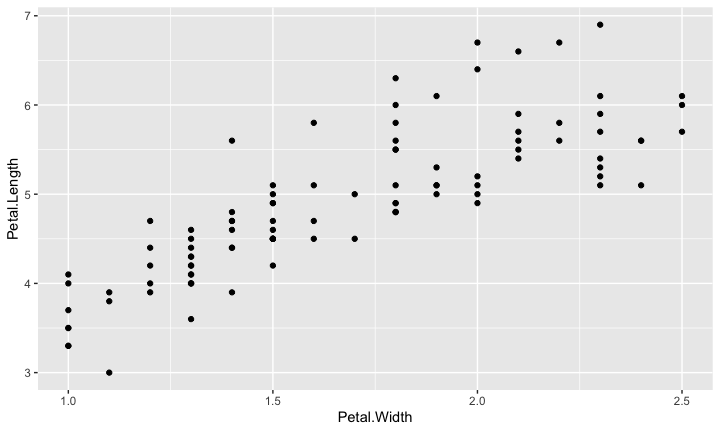
\includegraphics{eda5_files/figure-latex/unnamed-chunk-3-1.pdf}

\begin{center}\rule{0.5\linewidth}{0.5pt}\end{center}

\begin{Shaded}
\begin{Highlighting}[]
\NormalTok{df0 }\SpecialCharTok{\%\textgreater{}\%} \FunctionTok{ggplot}\NormalTok{(}\FunctionTok{aes}\NormalTok{(Petal.Width, Petal.Length)) }\SpecialCharTok{+} \FunctionTok{geom\_point}\NormalTok{() }\SpecialCharTok{+} \FunctionTok{geom\_smooth}\NormalTok{(}\AttributeTok{method=}\StringTok{"lm"}\NormalTok{,}\AttributeTok{formula=}\NormalTok{y}\SpecialCharTok{\textasciitilde{}}\NormalTok{x, }\AttributeTok{se=}\ConstantTok{FALSE}\NormalTok{)}
\end{Highlighting}
\end{Shaded}

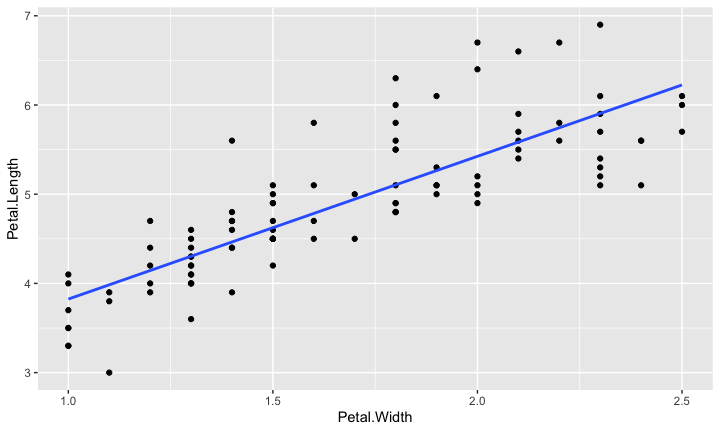
\includegraphics{eda5_files/figure-latex/unnamed-chunk-4-1.pdf}

\begin{center}\rule{0.5\linewidth}{0.5pt}\end{center}

\begin{Shaded}
\begin{Highlighting}[]
\NormalTok{df0 }\SpecialCharTok{\%\textgreater{}\%} \FunctionTok{ggplot}\NormalTok{(}\FunctionTok{aes}\NormalTok{(Sepal.Width, Sepal.Length)) }\SpecialCharTok{+} \FunctionTok{geom\_point}\NormalTok{()}
\end{Highlighting}
\end{Shaded}

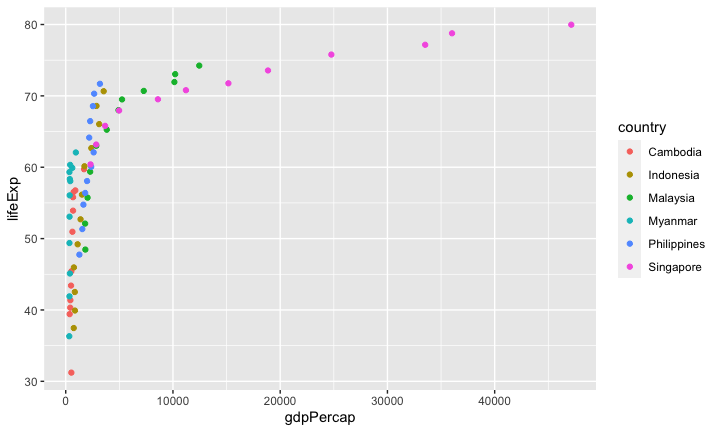
\includegraphics{eda5_files/figure-latex/unnamed-chunk-5-1.pdf}

\begin{center}\rule{0.5\linewidth}{0.5pt}\end{center}

\begin{Shaded}
\begin{Highlighting}[]
\NormalTok{df0 }\SpecialCharTok{\%\textgreater{}\%} \FunctionTok{ggplot}\NormalTok{(}\FunctionTok{aes}\NormalTok{(Sepal.Width, Sepal.Length)) }\SpecialCharTok{+} \FunctionTok{geom\_point}\NormalTok{() }\SpecialCharTok{+} \FunctionTok{geom\_smooth}\NormalTok{(}\AttributeTok{method=}\StringTok{"lm"}\NormalTok{,}\AttributeTok{formula=}\NormalTok{y}\SpecialCharTok{\textasciitilde{}}\NormalTok{x, }\AttributeTok{se=}\ConstantTok{FALSE}\NormalTok{)}
\end{Highlighting}
\end{Shaded}

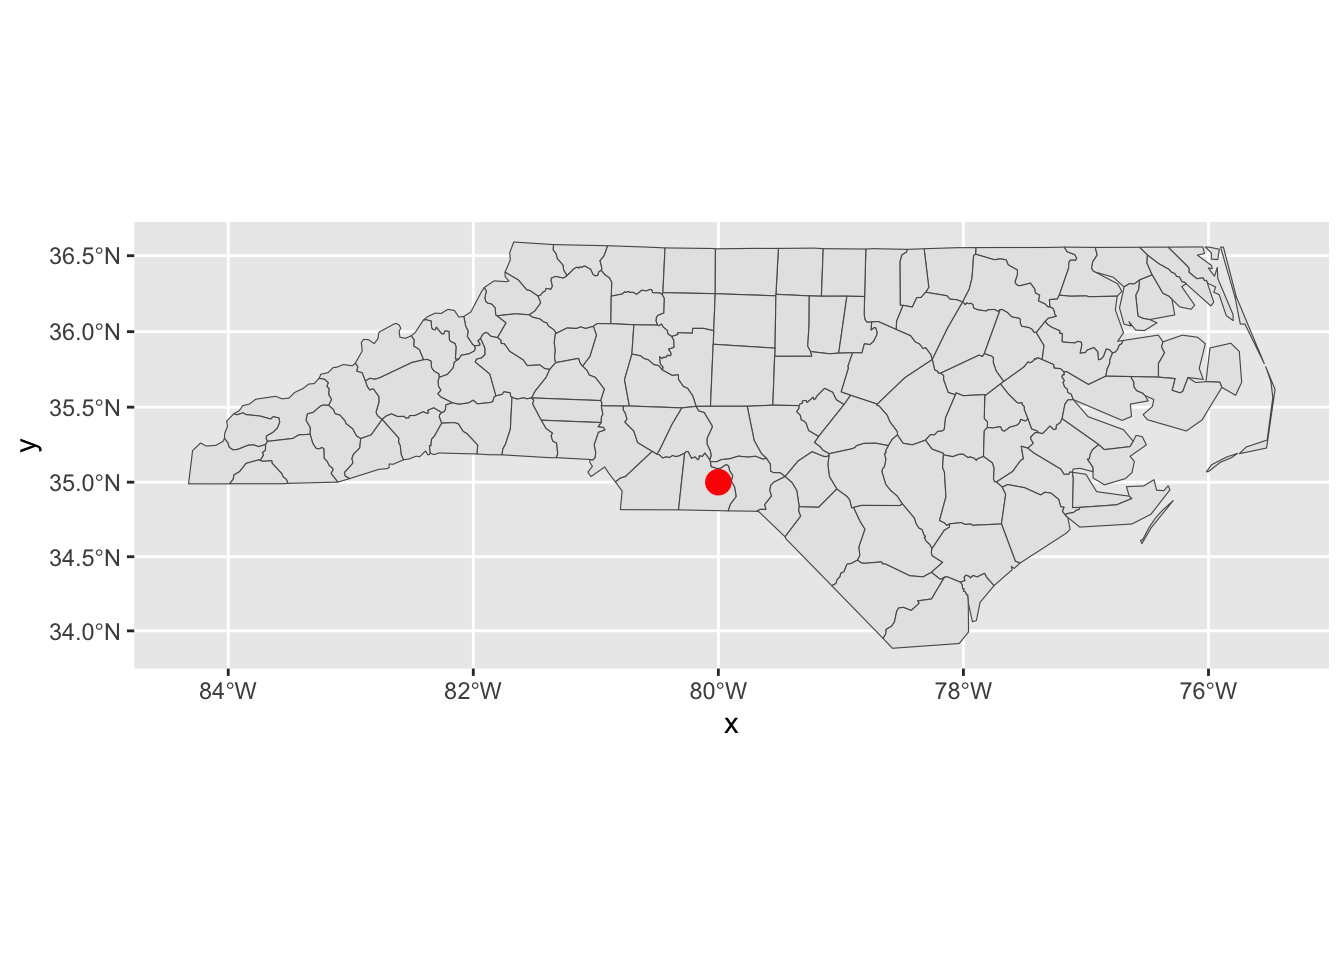
\includegraphics{eda5_files/figure-latex/unnamed-chunk-6-1.pdf}

\begin{center}\rule{0.5\linewidth}{0.5pt}\end{center}

\hypertarget{linear-model-petal.length-petal.width}{%
\subsubsection{Linear Model: Petal.Length \textasciitilde{}
Petal.Width}\label{linear-model-petal.length-petal.width}}

\begin{Shaded}
\begin{Highlighting}[]
\NormalTok{df0 }\SpecialCharTok{\%\textgreater{}\%} \FunctionTok{lm}\NormalTok{(Petal.Length }\SpecialCharTok{\textasciitilde{}}\NormalTok{ Petal.Width, .)}
\end{Highlighting}
\end{Shaded}

\begin{verbatim}
## 
## Call:
## lm(formula = Petal.Length ~ Petal.Width, data = .)
## 
## Coefficients:
## (Intercept)  Petal.Width  
##       2.224        1.600
\end{verbatim}

\begin{center}\rule{0.5\linewidth}{0.5pt}\end{center}

\hypertarget{formula-textpetal.length-2.224-1.600cdot-textpetal.width}{%
\subsubsection{\texorpdfstring{Formula:
\(\text{Petal.Length} = 2.224 + 1.600\cdot \text{Petal.Width}\)}{Formula: \textbackslash text\{Petal.Length\} = 2.224 + 1.600\textbackslash cdot \textbackslash text\{Petal.Width\}}}\label{formula-textpetal.length-2.224-1.600cdot-textpetal.width}}

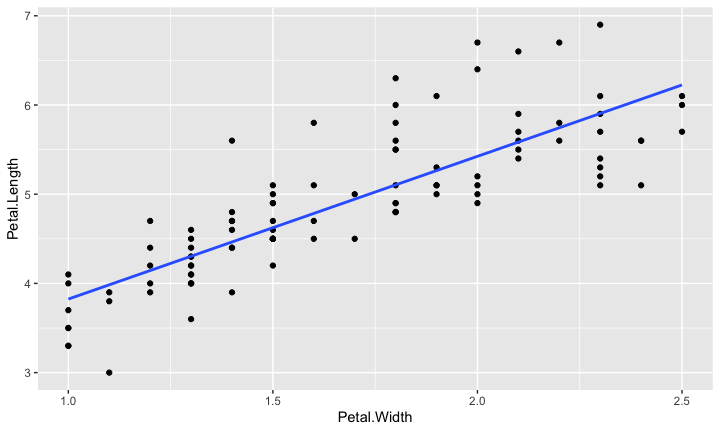
\includegraphics{eda5_files/figure-latex/unnamed-chunk-8-1.pdf}

\begin{center}\rule{0.5\linewidth}{0.5pt}\end{center}

\hypertarget{linear-model-sepal.length-sepal.width}{%
\subsubsection{Linear Model: Sepal.Length \textasciitilde{}
Sepal.Width}\label{linear-model-sepal.length-sepal.width}}

\begin{Shaded}
\begin{Highlighting}[]
\NormalTok{df0 }\SpecialCharTok{\%\textgreater{}\%} \FunctionTok{lm}\NormalTok{(Sepal.Length }\SpecialCharTok{\textasciitilde{}}\NormalTok{ Sepal.Width, .)}
\end{Highlighting}
\end{Shaded}

\begin{verbatim}
## 
## Call:
## lm(formula = Sepal.Length ~ Sepal.Width, data = .)
## 
## Coefficients:
## (Intercept)  Sepal.Width  
##       3.093        1.103
\end{verbatim}

\begin{center}\rule{0.5\linewidth}{0.5pt}\end{center}

\hypertarget{formula-textsepal.length-3.093-1.103cdot-textsepal.width}{%
\subsubsection{\texorpdfstring{Formula:
\(\text{Sepal.Length} = 3.093 + 1.103\cdot \text{Sepal.Width}\)}{Formula: \textbackslash text\{Sepal.Length\} = 3.093 + 1.103\textbackslash cdot \textbackslash text\{Sepal.Width\}}}\label{formula-textsepal.length-3.093-1.103cdot-textsepal.width}}

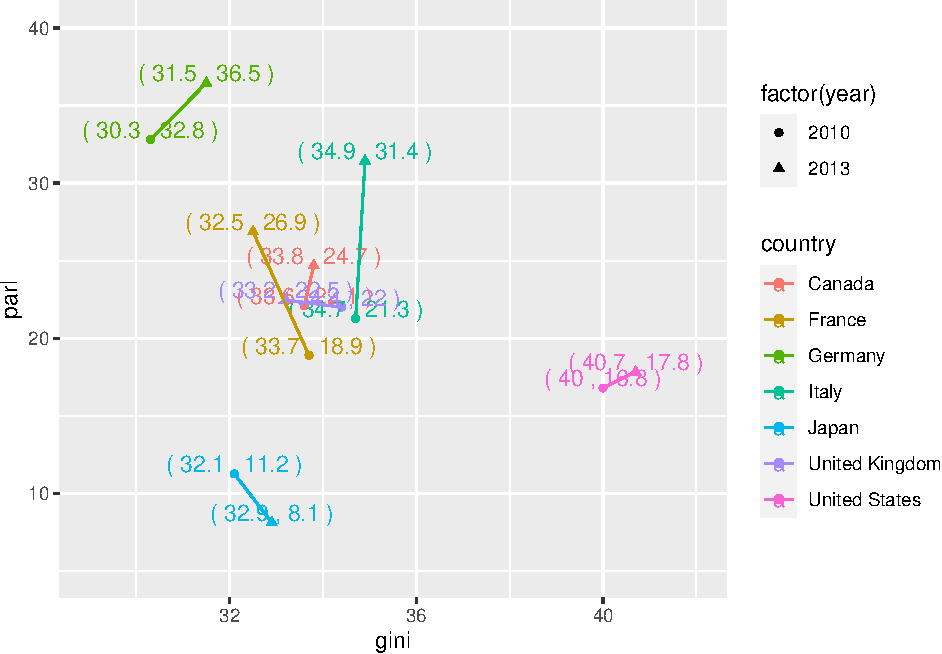
\includegraphics{eda5_files/figure-latex/unnamed-chunk-10-1.pdf}

\begin{center}\rule{0.5\linewidth}{0.5pt}\end{center}

\hypertarget{petal.length-petal.width-r-squared-0.6779---68}\label{petal.length-petal.width-r-squared-0.6779---68}}

\begin{Shaded}
\begin{Highlighting}[]
\NormalTok{df0 }\SpecialCharTok{\%\textgreater{}\%} \FunctionTok{lm}\NormalTok{(Petal.Length }\SpecialCharTok{\textasciitilde{}}\NormalTok{ Petal.Width, .) }\SpecialCharTok{\%\textgreater{}\%} \FunctionTok{summary}\NormalTok{()}
\end{Highlighting}
\end{Shaded}

\begin{verbatim}
## 
## Call:
## lm(formula = Petal.Length ~ Petal.Width, data = .)
## 
## Residuals:
##     Min      1Q  Median      3Q     Max 
## -0.9842 -0.3043 -0.1043  0.2407  1.2755 
## 
## Coefficients:
##             Estimate Std. Error t value Pr(>|t|)    
## (Intercept)   2.2240     0.1926   11.55   <2e-16 ***
## Petal.Width   1.6003     0.1114   14.36   <2e-16 ***
## ---
## Signif. codes:  0 '***' 0.001 '**' 0.01 '*' 0.05 '.' 0.1 ' ' 1
## 
## Residual standard error: 0.4709 on 98 degrees of freedom
## Multiple R-squared:  0.6779, Adjusted R-squared:  0.6746 
## F-statistic: 206.3 on 1 and 98 DF,  p-value: < 2.2e-16
\end{verbatim}

\begin{center}\rule{0.5\linewidth}{0.5pt}\end{center}

\hypertarget{sepal.length-sepal.width-r-squared-0.3068---31}\label{sepal.length-sepal.width-r-squared-0.3068---31}}

\begin{Shaded}
\begin{Highlighting}[]
\NormalTok{df0 }\SpecialCharTok{\%\textgreater{}\%} \FunctionTok{lm}\NormalTok{(Sepal.Length }\SpecialCharTok{\textasciitilde{}}\NormalTok{ Sepal.Width, .) }\SpecialCharTok{\%\textgreater{}\%} \FunctionTok{summary}\NormalTok{()}
\end{Highlighting}
\end{Shaded}

\begin{verbatim}
## 
## Call:
## lm(formula = Sepal.Length ~ Sepal.Width, data = .)
## 
## Residuals:
##     Min      1Q  Median      3Q     Max 
## -1.0032 -0.3877 -0.0774  0.3200  1.7381 
## 
## Coefficients:
##             Estimate Std. Error t value Pr(>|t|)    
## (Intercept)   3.0934     0.4844   6.387 5.70e-09 ***
## Sepal.Width   1.1033     0.1675   6.585 2.27e-09 ***
## ---
## Signif. codes:  0 '***' 0.001 '**' 0.01 '*' 0.05 '.' 0.1 ' ' 1
## 
## Residual standard error: 0.5547 on 98 degrees of freedom
## Multiple R-squared:  0.3068, Adjusted R-squared:  0.2997 
## F-statistic: 43.36 on 1 and 98 DF,  p-value: 2.27e-09
\end{verbatim}

\begin{center}\rule{0.5\linewidth}{0.5pt}\end{center}

\hypertarget{linear-model-basics-y-x}{%
\subsubsection{Linear Model Basics: y \textasciitilde{}
x}\label{linear-model-basics-y-x}}

\begin{verbatim}
lm(y~x, data)
\end{verbatim}

\begin{verbatim}
data %>% lm(y~x, .)
\end{verbatim}

y-intercept, and slope: rate of increase or decrease

\begin{verbatim}
summary(lm(y~x, data))
\end{verbatim}

\begin{verbatim}
data %>% lm(y~x, .) %>% summary()
\end{verbatim}

(Multiple) R Squared: a value between 0 and 1, strength of the model

\begin{center}\rule{0.5\linewidth}{0.5pt}\end{center}

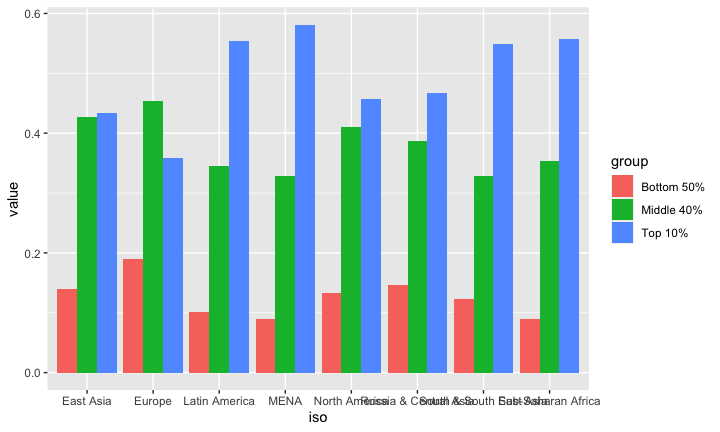
\includegraphics{eda5_files/figure-latex/unnamed-chunk-13-1.pdf}

\begin{center}\rule{0.5\linewidth}{0.5pt}\end{center}

\begin{Shaded}
\begin{Highlighting}[]
\NormalTok{df1 }\OtherTok{\textless{}{-}} \FunctionTok{data.frame}\NormalTok{(}\AttributeTok{x =} \FunctionTok{c}\NormalTok{(}\DecValTok{1}\NormalTok{,}\DecValTok{2}\NormalTok{,}\DecValTok{3}\NormalTok{,}\DecValTok{4}\NormalTok{), }\AttributeTok{y =} \FunctionTok{c}\NormalTok{(}\DecValTok{1}\NormalTok{,}\FloatTok{0.5}\NormalTok{,}\DecValTok{2}\NormalTok{, }\FloatTok{1.5}\NormalTok{))}
\NormalTok{ybar }\OtherTok{\textless{}{-}} \FunctionTok{mean}\NormalTok{(df1}\SpecialCharTok{$}\NormalTok{y)}
\NormalTok{mod1 }\OtherTok{\textless{}{-}} \FunctionTok{lm}\NormalTok{(y}\SpecialCharTok{\textasciitilde{}}\NormalTok{x, df1)}
\FunctionTok{augment}\NormalTok{(mod1) }\SpecialCharTok{\%\textgreater{}\%} \FunctionTok{ggplot}\NormalTok{() }\SpecialCharTok{+} \FunctionTok{geom\_point}\NormalTok{(}\FunctionTok{aes}\NormalTok{(x,y)) }\SpecialCharTok{+} \FunctionTok{geom\_smooth}\NormalTok{(}\FunctionTok{aes}\NormalTok{(x,y), }\AttributeTok{formula =}\NormalTok{ y}\SpecialCharTok{\textasciitilde{}}\NormalTok{x, }\AttributeTok{method =} \StringTok{"lm"}\NormalTok{, }\AttributeTok{se =} \ConstantTok{FALSE}\NormalTok{) }\SpecialCharTok{+} \FunctionTok{geom\_hline}\NormalTok{(}\AttributeTok{yintercept =}\NormalTok{ ybar, }\AttributeTok{linetype=}\StringTok{"longdash"}\NormalTok{, }\AttributeTok{col =} \StringTok{"red"}\NormalTok{) }\SpecialCharTok{+} \FunctionTok{geom\_point}\NormalTok{(}\FunctionTok{aes}\NormalTok{(x, ybar), }\AttributeTok{shape=}\DecValTok{4}\NormalTok{) }\SpecialCharTok{+} \FunctionTok{geom\_point}\NormalTok{(}\FunctionTok{aes}\NormalTok{(x, .fitted), }\AttributeTok{shape =}\DecValTok{9}\NormalTok{, }\AttributeTok{size=}\DecValTok{2}\NormalTok{) }\SpecialCharTok{+} \FunctionTok{geom\_text}\NormalTok{(}\FunctionTok{aes}\NormalTok{(x, ybar, }\AttributeTok{label =} \FunctionTok{paste0}\NormalTok{(}\StringTok{"("}\NormalTok{,x,}\StringTok{","}\NormalTok{,}\FloatTok{1.25}\NormalTok{,}\StringTok{")"}\NormalTok{)), }\AttributeTok{nudge\_y =} \SpecialCharTok{{-}}\FloatTok{0.1}\NormalTok{, }\AttributeTok{col =} \StringTok{"red"}\NormalTok{) }\SpecialCharTok{+} \FunctionTok{geom\_text}\NormalTok{(}\FunctionTok{aes}\NormalTok{(x, .fitted, }\AttributeTok{label =} \FunctionTok{paste0}\NormalTok{(}\StringTok{"("}\NormalTok{,x,}\StringTok{","}\NormalTok{,.fitted,}\StringTok{")"}\NormalTok{)), }\AttributeTok{nudge\_y =} \SpecialCharTok{{-}}\FloatTok{0.1}\NormalTok{, }\AttributeTok{col =} \StringTok{"blue"}\NormalTok{) }\SpecialCharTok{+} \FunctionTok{geom\_text}\NormalTok{(}\FunctionTok{aes}\NormalTok{(x, y, }\AttributeTok{label =} \FunctionTok{paste0}\NormalTok{(}\StringTok{"("}\NormalTok{,x,}\StringTok{","}\NormalTok{,y,}\StringTok{")"}\NormalTok{)), }\AttributeTok{nudge\_y =} \SpecialCharTok{{-}}\FloatTok{0.1}\NormalTok{) }
\end{Highlighting}
\end{Shaded}

\begin{itemize}
\tightlist
\item
  \((x_1, y_1)\), \((x_2,y_2)\), \((x_3, y_3)\), \((x_4, y_4)\): Data
  points
\item
  \(\bar{y}\): mean of y = \((y_1 + y_2 + y_3 + y_4)/4\).
\item
  \(\hat{y}_i\): prediction at \(x_i\),

  \begin{itemize}
  \tightlist
  \item
    \((x_1, \hat{y}_1)\), \((x_2, \hat{y}_2)\), \((x_3, \hat{y}_3)\),
    \((x_4, \hat{y}_4)\) are on the regression line.
  \end{itemize}
\item
  \(y_1-\hat{y}_1\), \(y_2-\hat{y}_2\), \(y_2-\hat{y}_2\),
  \(y_2-\hat{y}_2\) are called residues.
\end{itemize}

\begin{center}\rule{0.5\linewidth}{0.5pt}\end{center}

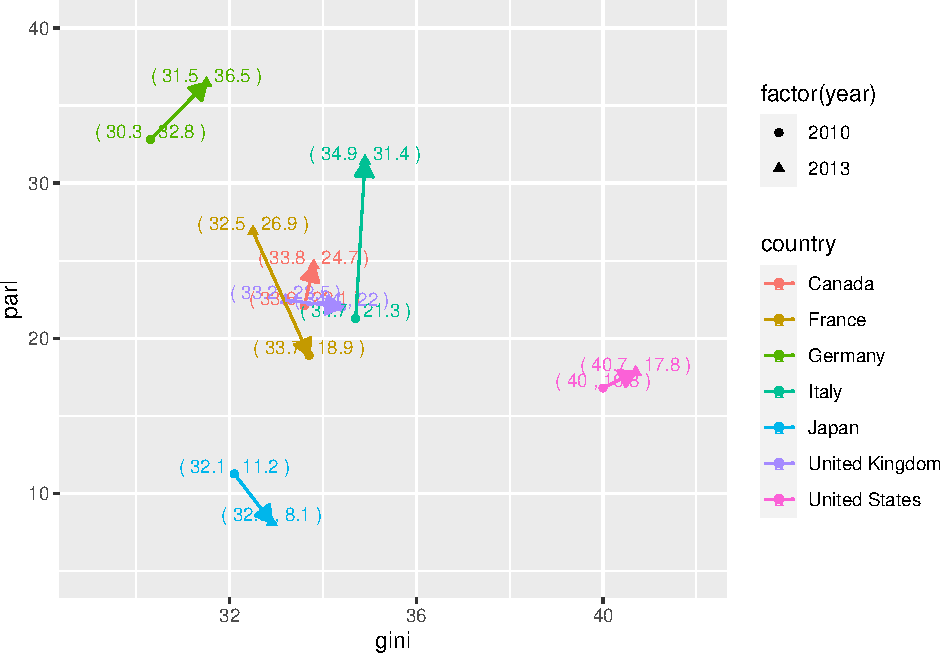
\includegraphics{eda5_files/figure-latex/unnamed-chunk-15-1.pdf}

\begin{center}\rule{0.5\linewidth}{0.5pt}\end{center}

\hypertarget{r-squared}{%
\subsubsection{R Squared}\label{r-squared}}

\[SS_{tot} = (1-1.25)^2 + (0.5-1.25)^2 + (2-1.25)^2 + (1.5-1.25)^2 = 1.25\]
\[SS_{res} = (1-0.8)^2 + (0.5-1.1)^2 + (2-1.4)^2 + (1.5-1.7)^2 = 0.8\]
\[R^2 = 1 - \frac{SS_{res}}{SS_{tot}} = 1- \frac{0.8}{1.25} = 0.36.\]

\begin{center}\rule{0.5\linewidth}{0.5pt}\end{center}

\begin{Shaded}
\begin{Highlighting}[]
\FunctionTok{summary}\NormalTok{(mod1)}\SpecialCharTok{$}\NormalTok{r.squared}
\end{Highlighting}
\end{Shaded}

\begin{verbatim}
## [1] 0.36
\end{verbatim}

\begin{Shaded}
\begin{Highlighting}[]
\NormalTok{mod1 }\SpecialCharTok{\%\textgreater{}\%} \FunctionTok{glance}\NormalTok{() }\SpecialCharTok{\%\textgreater{}\%} \FunctionTok{pull}\NormalTok{(r.squared)}
\end{Highlighting}
\end{Shaded}

\begin{verbatim}
## [1] 0.36
\end{verbatim}

\begin{Shaded}
\begin{Highlighting}[]
\NormalTok{mod1 }\SpecialCharTok{\%\textgreater{}\%} \FunctionTok{glance}\NormalTok{() }\SpecialCharTok{\%\textgreater{}\%} \FunctionTok{select}\NormalTok{(}\StringTok{\textasciigrave{}}\AttributeTok{R Squared}\StringTok{\textasciigrave{}} \OtherTok{=}\NormalTok{ r.squared)}
\end{Highlighting}
\end{Shaded}

\begin{verbatim}
## # A tibble: 1 x 1
##   `R Squared`
##         <dbl>
## 1        0.36
\end{verbatim}

\begin{center}\rule{0.5\linewidth}{0.5pt}\end{center}

\begin{Shaded}
\begin{Highlighting}[]
\NormalTok{mod1 }\SpecialCharTok{\%\textgreater{}\%} \FunctionTok{summary}\NormalTok{() }\SpecialCharTok{\%\textgreater{}\%} \FunctionTok{glimpse}\NormalTok{()}
\end{Highlighting}
\end{Shaded}

\begin{verbatim}
## List of 11
##  $ call         : language lm(formula = y ~ x, data = df1)
##  $ terms        :Classes 'terms', 'formula'  language y ~ x
##   .. ..- attr(*, "variables")= language list(y, x)
##   .. ..- attr(*, "factors")= int [1:2, 1] 0 1
##   .. .. ..- attr(*, "dimnames")=List of 2
##   .. ..- attr(*, "term.labels")= chr "x"
##   .. ..- attr(*, "order")= int 1
##   .. ..- attr(*, "intercept")= int 1
##   .. ..- attr(*, "response")= int 1
##   .. ..- attr(*, ".Environment")=<environment: R_GlobalEnv> 
##   .. ..- attr(*, "predvars")= language list(y, x)
##   .. ..- attr(*, "dataClasses")= Named chr [1:2] "numeric" "numeric"
##   .. .. ..- attr(*, "names")= chr [1:2] "y" "x"
##  $ residuals    : Named num [1:4] 0.2 -0.6 0.6 -0.2
##   ..- attr(*, "names")= chr [1:4] "1" "2" "3" "4"
##  $ coefficients : num [1:2, 1:4] 0.5 0.3 0.775 0.283 0.645 ...
##   ..- attr(*, "dimnames")=List of 2
##   .. ..$ : chr [1:2] "(Intercept)" "x"
##   .. ..$ : chr [1:4] "Estimate" "Std. Error" "t value" "Pr(>|t|)"
##  $ aliased      : Named logi [1:2] FALSE FALSE
##   ..- attr(*, "names")= chr [1:2] "(Intercept)" "x"
##  $ sigma        : num 0.632
##  $ df           : int [1:3] 2 2 2
##  $ r.squared    : num 0.36
##  $ adj.r.squared: num 0.04
##  $ fstatistic   : Named num [1:3] 1.12 1 2
##   ..- attr(*, "names")= chr [1:3] "value" "numdf" "dendf"
##  $ cov.unscaled : num [1:2, 1:2] 1.5 -0.5 -0.5 0.2
##   ..- attr(*, "dimnames")=List of 2
##   .. ..$ : chr [1:2] "(Intercept)" "x"
##   .. ..$ : chr [1:2] "(Intercept)" "x"
##  - attr(*, "class")= chr "summary.lm"
\end{verbatim}

\begin{center}\rule{0.5\linewidth}{0.5pt}\end{center}

\hypertarget{useful-mathematical-formula}{%
\subsubsection{Useful Mathematical
Formula}\label{useful-mathematical-formula}}

\begin{itemize}
\tightlist
\item
  Let \(x = c(x_1, x_2, \ldots, x_n)\) be the independent variable,
  i.e., Sepal.L
\item
  Let \(y = c(y_1, y_2, \ldots, y_n)\) be the dependent variable, i.e.,
  Sepal.W
\item
  Let \(\mbox{pred} = c(\hat{y}_1, \hat{y}_2, \ldots, \hat{y}_n)\) be
  the predicted values by linear regression.
\end{itemize}

\begin{align}
\mbox{slope of the regression line}  &= \frac{cov(x,y)}{var(x)} = \frac{cor(x,y)\sqrt{var(y)}}{\sqrt{var(x)}}\\
\mbox{total sum of squares} &= SS_{tot} = \sum_{i}(y_i-mean(y))^2\\
\mbox{residual sum of squares} &= SS_{res} = \sum_{i}(y_i-\mbox{pred}_i)^2 = \sum_{i}(y_i-\hat{y}_i)^2\\
\mbox{R squared} = R^2 & = 1 - \frac{SS_{res}}{SS_{tot}} = cor(x,y)^2
\end{align}

\hypertarget{adjusted-r-squared}{%
\subsubsection{Adjusted R Squared}\label{adjusted-r-squared}}

\[\text{Adjusted }R^2 = 1- \frac{(1-R^2)(n-1)}{n-k-1}\] \(n\): number of
observations, the number of rows

\(k\): number of variables used for prediction

\begin{center}\rule{0.5\linewidth}{0.5pt}\end{center}

\begin{Shaded}
\begin{Highlighting}[]
\NormalTok{df0 }\SpecialCharTok{\%\textgreater{}\%} \FunctionTok{select}\NormalTok{(}\DecValTok{1}\SpecialCharTok{:}\DecValTok{4}\NormalTok{) }\SpecialCharTok{\%\textgreater{}\%} \FunctionTok{cor}\NormalTok{()}
\end{Highlighting}
\end{Shaded}

\begin{verbatim}
##              Sepal.Length Sepal.Width Petal.Length Petal.Width
## Sepal.Length    1.0000000   0.5538548    0.8284787   0.5937094
## Sepal.Width     0.5538548   1.0000000    0.5198023   0.5662025
## Petal.Length    0.8284787   0.5198023    1.0000000   0.8233476
## Petal.Width     0.5937094   0.5662025    0.8233476   1.0000000
\end{verbatim}

\begin{Shaded}
\begin{Highlighting}[]
\NormalTok{cormat }\OtherTok{\textless{}{-}}\NormalTok{ df0 }\SpecialCharTok{\%\textgreater{}\%} \FunctionTok{select}\NormalTok{(}\DecValTok{1}\SpecialCharTok{:}\DecValTok{4}\NormalTok{) }\SpecialCharTok{\%\textgreater{}\%} \FunctionTok{cor}\NormalTok{()}
\NormalTok{cormat}\SpecialCharTok{*}\NormalTok{cormat}
\end{Highlighting}
\end{Shaded}

\begin{verbatim}
##              Sepal.Length Sepal.Width Petal.Length Petal.Width
## Sepal.Length    1.0000000   0.3067552    0.6863769   0.3524909
## Sepal.Width     0.3067552   1.0000000    0.2701944   0.3205853
## Petal.Length    0.6863769   0.2701944    1.0000000   0.6779013
## Petal.Width     0.3524909   0.3205853    0.6779013   1.0000000
\end{verbatim}

\begin{center}\rule{0.5\linewidth}{0.5pt}\end{center}

\begin{Shaded}
\begin{Highlighting}[]
\FunctionTok{as\_tibble}\NormalTok{(iris) }\SpecialCharTok{\%\textgreater{}\%} \FunctionTok{filter}\NormalTok{(Species }\SpecialCharTok{==} \StringTok{"setosa"}\NormalTok{) }\SpecialCharTok{\%\textgreater{}\%} \FunctionTok{select}\NormalTok{(}\SpecialCharTok{{-}}\DecValTok{5}\NormalTok{) }\SpecialCharTok{\%\textgreater{}\%} \FunctionTok{cor}\NormalTok{()}
\end{Highlighting}
\end{Shaded}

\begin{verbatim}
##              Sepal.Length Sepal.Width Petal.Length Petal.Width
## Sepal.Length    1.0000000   0.7425467    0.2671758   0.2780984
## Sepal.Width     0.7425467   1.0000000    0.1777000   0.2327520
## Petal.Length    0.2671758   0.1777000    1.0000000   0.3316300
## Petal.Width     0.2780984   0.2327520    0.3316300   1.0000000
\end{verbatim}

\begin{Shaded}
\begin{Highlighting}[]
\FunctionTok{as\_tibble}\NormalTok{(iris) }\SpecialCharTok{\%\textgreater{}\%} \FunctionTok{filter}\NormalTok{(Species }\SpecialCharTok{==} \StringTok{"virginica"}\NormalTok{) }\SpecialCharTok{\%\textgreater{}\%} \FunctionTok{select}\NormalTok{(}\SpecialCharTok{{-}}\DecValTok{5}\NormalTok{) }\SpecialCharTok{\%\textgreater{}\%} \FunctionTok{cor}\NormalTok{()}
\end{Highlighting}
\end{Shaded}

\begin{verbatim}
##              Sepal.Length Sepal.Width Petal.Length Petal.Width
## Sepal.Length    1.0000000   0.4572278    0.8642247   0.2811077
## Sepal.Width     0.4572278   1.0000000    0.4010446   0.5377280
## Petal.Length    0.8642247   0.4010446    1.0000000   0.3221082
## Petal.Width     0.2811077   0.5377280    0.3221082   1.0000000
\end{verbatim}

\begin{Shaded}
\begin{Highlighting}[]
\FunctionTok{as\_tibble}\NormalTok{(iris) }\SpecialCharTok{\%\textgreater{}\%} \FunctionTok{filter}\NormalTok{(Species }\SpecialCharTok{==} \StringTok{"versicolor"}\NormalTok{) }\SpecialCharTok{\%\textgreater{}\%} \FunctionTok{select}\NormalTok{(}\SpecialCharTok{{-}}\DecValTok{5}\NormalTok{) }\SpecialCharTok{\%\textgreater{}\%} \FunctionTok{cor}\NormalTok{()}
\end{Highlighting}
\end{Shaded}

\begin{verbatim}
##              Sepal.Length Sepal.Width Petal.Length Petal.Width
## Sepal.Length    1.0000000   0.5259107    0.7540490   0.5464611
## Sepal.Width     0.5259107   1.0000000    0.5605221   0.6639987
## Petal.Length    0.7540490   0.5605221    1.0000000   0.7866681
## Petal.Width     0.5464611   0.6639987    0.7866681   1.0000000
\end{verbatim}

\begin{center}\rule{0.5\linewidth}{0.5pt}\end{center}

\begin{Shaded}
\begin{Highlighting}[]
\FunctionTok{as\_tibble}\NormalTok{(iris) }\SpecialCharTok{\%\textgreater{}\%} \FunctionTok{filter}\NormalTok{(Species }\SpecialCharTok{==} \StringTok{"virginica"}\NormalTok{) }\SpecialCharTok{\%\textgreater{}\%} \FunctionTok{ggplot}\NormalTok{(}\FunctionTok{aes}\NormalTok{(Sepal.Length, Petal.Length)) }\SpecialCharTok{+} \FunctionTok{geom\_point}\NormalTok{() }\SpecialCharTok{+} \FunctionTok{geom\_smooth}\NormalTok{(}\AttributeTok{method =} \StringTok{"lm"}\NormalTok{, }\AttributeTok{formula =}\NormalTok{ y}\SpecialCharTok{\textasciitilde{}}\NormalTok{x, }\AttributeTok{se =} \ConstantTok{FALSE}\NormalTok{)}
\end{Highlighting}
\end{Shaded}

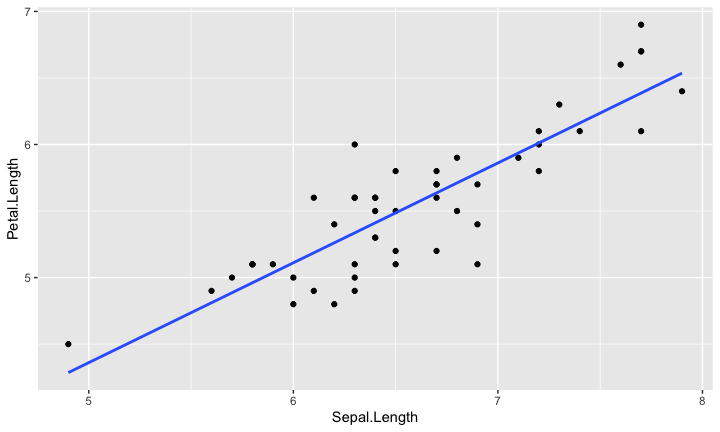
\includegraphics{eda5_files/figure-latex/unnamed-chunk-25-1.pdf}

\begin{center}\rule{0.5\linewidth}{0.5pt}\end{center}

\begin{Shaded}
\begin{Highlighting}[]
\FunctionTok{as\_tibble}\NormalTok{(iris) }\SpecialCharTok{\%\textgreater{}\%} \FunctionTok{filter}\NormalTok{(Species }\SpecialCharTok{==} \StringTok{"virginica"}\NormalTok{) }\SpecialCharTok{\%\textgreater{}\%} \FunctionTok{lm}\NormalTok{(Petal.Length }\SpecialCharTok{\textasciitilde{}}\NormalTok{ Sepal.Length, .) }\SpecialCharTok{\%\textgreater{}\%} \FunctionTok{glance}\NormalTok{() }\SpecialCharTok{\%\textgreater{}\%} \FunctionTok{pull}\NormalTok{(r.squared) }\SpecialCharTok{\%\textgreater{}\%} \FunctionTok{sqrt}\NormalTok{()}
\end{Highlighting}
\end{Shaded}

\begin{verbatim}
## [1] 0.8642247
\end{verbatim}

Correlations of the data suggest the possible strength of linear model y
\textasciitilde{} x.

\begin{Shaded}
\begin{Highlighting}[]
\NormalTok{iris }\SpecialCharTok{\%\textgreater{}\%} \FunctionTok{select}\NormalTok{(}\SpecialCharTok{{-}}\DecValTok{5}\NormalTok{) }\SpecialCharTok{\%\textgreater{}\%} \FunctionTok{cor}\NormalTok{()}
\end{Highlighting}
\end{Shaded}

\begin{verbatim}
##              Sepal.Length Sepal.Width Petal.Length Petal.Width
## Sepal.Length    1.0000000  -0.1175698    0.8717538   0.8179411
## Sepal.Width    -0.1175698   1.0000000   -0.4284401  -0.3661259
## Petal.Length    0.8717538  -0.4284401    1.0000000   0.9628654
## Petal.Width     0.8179411  -0.3661259    0.9628654   1.0000000
\end{verbatim}

\begin{center}\rule{0.5\linewidth}{0.5pt}\end{center}

\hypertarget{examples-wdi}{%
\subsubsection{Examples: WDI}\label{examples-wdi}}

\begin{itemize}
\tightlist
\item
  SP.DYN.LE00.IN: Life expectancy at birth, total (years)
\end{itemize}

\begin{Shaded}
\begin{Highlighting}[]
\NormalTok{wdi\_lifeExp }\OtherTok{\textless{}{-}} \FunctionTok{WDI}\NormalTok{(}\AttributeTok{indicator =} \FunctionTok{c}\NormalTok{(}\AttributeTok{lifeExp =} \StringTok{"SP.DYN.LE00.IN"}\NormalTok{))}
\end{Highlighting}
\end{Shaded}

\begin{verbatim}
## Rows: 16492 Columns: 5
## -- Column specification --------------------------------------------------------
## Delimiter: ","
## chr (3): country, iso2c, iso3c
## dbl (2): year, lifeExp
## 
## i Use `spec()` to retrieve the full column specification for this data.
## i Specify the column types or set `show_col_types = FALSE` to quiet this message.
\end{verbatim}

\begin{center}\rule{0.5\linewidth}{0.5pt}\end{center}

\begin{Shaded}
\begin{Highlighting}[]
\NormalTok{wdi\_lifeExp }\SpecialCharTok{\%\textgreater{}\%} \FunctionTok{filter}\NormalTok{(country }\SpecialCharTok{==} \StringTok{"World"}\NormalTok{) }\SpecialCharTok{\%\textgreater{}\%} \FunctionTok{drop\_na}\NormalTok{(lifeExp) }\SpecialCharTok{\%\textgreater{}\%}
  \FunctionTok{ggplot}\NormalTok{(}\FunctionTok{aes}\NormalTok{(year, lifeExp)) }\SpecialCharTok{+} \FunctionTok{geom\_point}\NormalTok{() }\SpecialCharTok{+} \FunctionTok{geom\_smooth}\NormalTok{(}\AttributeTok{method =} \StringTok{"lm"}\NormalTok{, }\AttributeTok{se =} \ConstantTok{FALSE}\NormalTok{)}
\end{Highlighting}
\end{Shaded}

\begin{verbatim}
## `geom_smooth()` using formula = 'y ~ x'
\end{verbatim}

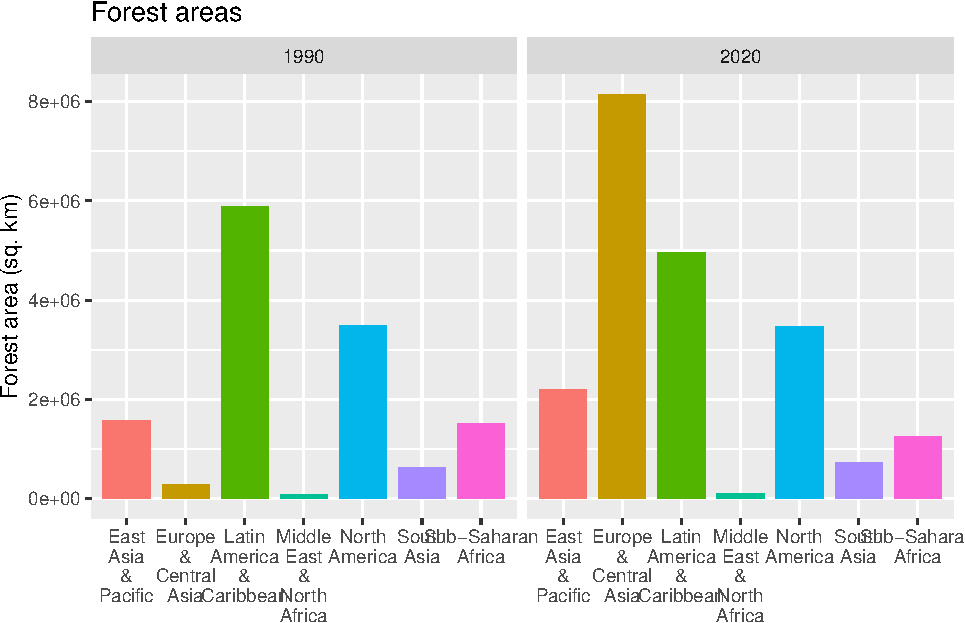
\includegraphics{eda5_files/figure-latex/unnamed-chunk-31-1.pdf}

\begin{center}\rule{0.5\linewidth}{0.5pt}\end{center}

\begin{Shaded}
\begin{Highlighting}[]
\NormalTok{wdi\_lifeExp }\SpecialCharTok{\%\textgreater{}\%} \FunctionTok{lm}\NormalTok{(lifeExp }\SpecialCharTok{\textasciitilde{}}\NormalTok{ year, .) }\SpecialCharTok{\%\textgreater{}\%} \FunctionTok{summary}\NormalTok{()}
\end{Highlighting}
\end{Shaded}

\begin{verbatim}
## 
## Call:
## lm(formula = lifeExp ~ year, data = .)
## 
## Residuals:
##     Min      1Q  Median      3Q     Max 
## -51.142  -7.297   1.782   7.873  19.139 
## 
## Coefficients:
##               Estimate Std. Error t value Pr(>|t|)    
## (Intercept) -5.574e+02  8.987e+00  -62.02   <2e-16 ***
## year         3.123e-01  4.515e-03   69.15   <2e-16 ***
## ---
## Signif. codes:  0 '***' 0.001 '**' 0.01 '*' 0.05 '.' 0.1 ' ' 1
## 
## Residual standard error: 9.797 on 15202 degrees of freedom
##   (1288 observations deleted due to missingness)
## Multiple R-squared:  0.2393, Adjusted R-squared:  0.2392 
## F-statistic:  4782 on 1 and 15202 DF,  p-value: < 2.2e-16
\end{verbatim}

\[lifeExp \sim -557.4 + 0.3123 \cdot year\] Each year, life expectancy
at birth increases approximately 0.3123 years. R-squared of this model
is 0.2392, and the model explains 24\%.

\begin{center}\rule{0.5\linewidth}{0.5pt}\end{center}

\begin{Shaded}
\begin{Highlighting}[]
\NormalTok{wdi\_lifeExp }\SpecialCharTok{\%\textgreater{}\%} \FunctionTok{filter}\NormalTok{(country }\SpecialCharTok{==} \StringTok{"World"}\NormalTok{, year }\SpecialCharTok{\textgreater{}=} \DecValTok{1962}\NormalTok{, year }\SpecialCharTok{\textless{}=} \DecValTok{2019}\NormalTok{) }\SpecialCharTok{\%\textgreater{}\%} \FunctionTok{drop\_na}\NormalTok{(lifeExp) }\SpecialCharTok{\%\textgreater{}\%} \FunctionTok{lm}\NormalTok{(lifeExp }\SpecialCharTok{\textasciitilde{}}\NormalTok{ year, .) }\SpecialCharTok{\%\textgreater{}\%} \FunctionTok{summary}\NormalTok{()}
\end{Highlighting}
\end{Shaded}

\begin{verbatim}
## 
## Call:
## lm(formula = lifeExp ~ year, data = .)
## 
## Residuals:
##      Min       1Q   Median       3Q      Max 
## -1.01769 -0.29535 -0.04302  0.38542  0.82106 
## 
## Coefficients:
##               Estimate Std. Error t value Pr(>|t|)    
## (Intercept) -5.543e+02  7.885e+00  -70.30   <2e-16 ***
## year         3.110e-01  3.961e-03   78.52   <2e-16 ***
## ---
## Signif. codes:  0 '***' 0.001 '**' 0.01 '*' 0.05 '.' 0.1 ' ' 1
## 
## Residual standard error: 0.505 on 56 degrees of freedom
## Multiple R-squared:  0.991,  Adjusted R-squared:  0.9908 
## F-statistic:  6166 on 1 and 56 DF,  p-value: < 2.2e-16
\end{verbatim}

\begin{center}\rule{0.5\linewidth}{0.5pt}\end{center}

\hypertarget{brics}{%
\subsubsection{BRICs}\label{brics}}

\begin{Shaded}
\begin{Highlighting}[]
\NormalTok{mod\_brics }\OtherTok{\textless{}{-}}\NormalTok{ wdi\_lifeExp }\SpecialCharTok{\%\textgreater{}\%} \FunctionTok{filter}\NormalTok{(country }\SpecialCharTok{\%in\%} \FunctionTok{c}\NormalTok{(}\StringTok{"Brazil"}\NormalTok{, }\StringTok{"Russian Federation"}\NormalTok{, }\StringTok{"India"}\NormalTok{, }\StringTok{"China"}\NormalTok{)) }\SpecialCharTok{\%\textgreater{}\%} \FunctionTok{drop\_na}\NormalTok{(lifeExp) }\SpecialCharTok{\%\textgreater{}\%} \FunctionTok{lm}\NormalTok{(lifeExp }\SpecialCharTok{\textasciitilde{}}\NormalTok{ year, .) }\SpecialCharTok{\%\textgreater{}\%} \FunctionTok{summary}\NormalTok{()}
\NormalTok{mod\_brics}\SpecialCharTok{$}\NormalTok{r.squared}
\end{Highlighting}
\end{Shaded}

\begin{verbatim}
## [1] 0.5658162
\end{verbatim}

\begin{Shaded}
\begin{Highlighting}[]
\NormalTok{wdi\_lifeExp }\SpecialCharTok{\%\textgreater{}\%} \FunctionTok{filter}\NormalTok{(country }\SpecialCharTok{\%in\%} \FunctionTok{c}\NormalTok{(}\StringTok{"Brazil"}\NormalTok{, }\StringTok{"Russian Federation"}\NormalTok{, }\StringTok{"India"}\NormalTok{, }\StringTok{"China"}\NormalTok{)) }\SpecialCharTok{\%\textgreater{}\%} \FunctionTok{drop\_na}\NormalTok{(lifeExp) }\SpecialCharTok{\%\textgreater{}\%}
  \FunctionTok{ggplot}\NormalTok{(}\FunctionTok{aes}\NormalTok{(year, lifeExp)) }\SpecialCharTok{+} \FunctionTok{geom\_point}\NormalTok{() }\SpecialCharTok{+} \FunctionTok{geom\_smooth}\NormalTok{(}\AttributeTok{formula =}\NormalTok{ y}\SpecialCharTok{\textasciitilde{}}\NormalTok{x, }\AttributeTok{method =} \StringTok{"lm"}\NormalTok{, }\AttributeTok{se =} \ConstantTok{FALSE}\NormalTok{)}
\end{Highlighting}
\end{Shaded}

\begin{center}\rule{0.5\linewidth}{0.5pt}\end{center}

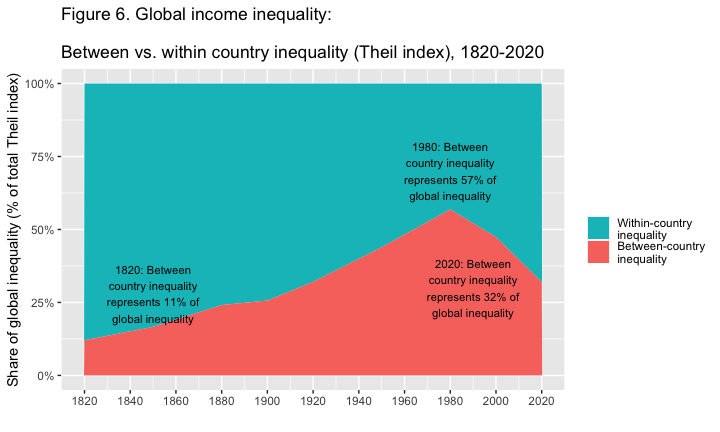
\includegraphics{eda5_files/figure-latex/unnamed-chunk-36-1.pdf}

\begin{center}\rule{0.5\linewidth}{0.5pt}\end{center}

\begin{Shaded}
\begin{Highlighting}[]
\NormalTok{wdi\_lifeExp }\SpecialCharTok{\%\textgreater{}\%} \FunctionTok{filter}\NormalTok{(country }\SpecialCharTok{\%in\%} \FunctionTok{c}\NormalTok{(}\StringTok{"Brazil"}\NormalTok{, }\StringTok{"Russian Federation"}\NormalTok{, }\StringTok{"India"}\NormalTok{, }\StringTok{"China"}\NormalTok{)) }\SpecialCharTok{\%\textgreater{}\%} \FunctionTok{drop\_na}\NormalTok{(lifeExp) }\SpecialCharTok{\%\textgreater{}\%}
  \FunctionTok{ggplot}\NormalTok{(}\FunctionTok{aes}\NormalTok{(year, lifeExp, }\AttributeTok{color =}\NormalTok{ country)) }\SpecialCharTok{+} \FunctionTok{geom\_point}\NormalTok{(}\FunctionTok{aes}\NormalTok{(}\AttributeTok{shape =}\NormalTok{ country)) }\SpecialCharTok{+} \FunctionTok{geom\_smooth}\NormalTok{(}\AttributeTok{formula =}\NormalTok{ y}\SpecialCharTok{\textasciitilde{}}\NormalTok{x, }\AttributeTok{method =} \StringTok{"lm"}\NormalTok{, }\AttributeTok{se =} \ConstantTok{FALSE}\NormalTok{)}
\end{Highlighting}
\end{Shaded}

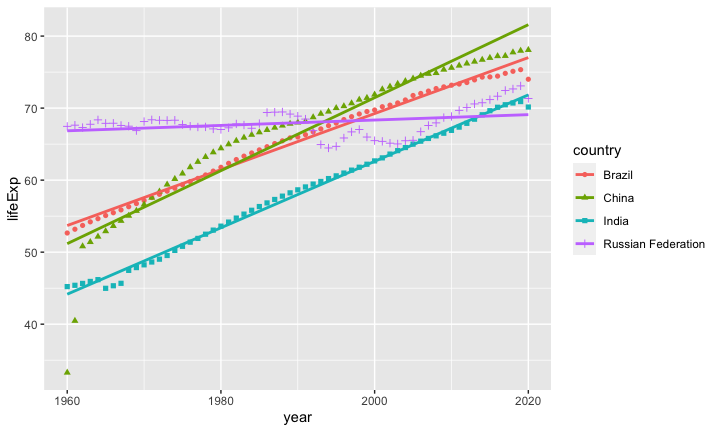
\includegraphics{eda5_files/figure-latex/unnamed-chunk-37-1.pdf}

\begin{center}\rule{0.5\linewidth}{0.5pt}\end{center}

\begin{Shaded}
\begin{Highlighting}[]
\NormalTok{country\_model }\OtherTok{\textless{}{-}} \ControlFlowTok{function}\NormalTok{(df) \{}
  \FunctionTok{lm}\NormalTok{(lifeExp }\SpecialCharTok{\textasciitilde{}}\NormalTok{ year, }\AttributeTok{data =}\NormalTok{ df)}
\NormalTok{\}}

\NormalTok{by\_country }\OtherTok{\textless{}{-}}\NormalTok{ wdi\_lifeExp }\SpecialCharTok{\%\textgreater{}\%} \FunctionTok{filter}\NormalTok{(country }\SpecialCharTok{\%in\%} \FunctionTok{c}\NormalTok{(}\StringTok{"Brazil"}\NormalTok{, }\StringTok{"Russian Federation"}\NormalTok{, }\StringTok{"India"}\NormalTok{, }\StringTok{"China"}\NormalTok{)) }\SpecialCharTok{\%\textgreater{}\%} \FunctionTok{drop\_na}\NormalTok{(lifeExp) }\SpecialCharTok{\%\textgreater{}\%} \FunctionTok{group\_by}\NormalTok{(country) }\SpecialCharTok{\%\textgreater{}\%} \FunctionTok{nest}\NormalTok{()}

\NormalTok{by\_country }\OtherTok{\textless{}{-}}\NormalTok{ by\_country }\SpecialCharTok{\%\textgreater{}\%} 
  \FunctionTok{mutate}\NormalTok{(}\AttributeTok{model =} \FunctionTok{map}\NormalTok{(data, country\_model))}

\NormalTok{by\_country }\SpecialCharTok{\%\textgreater{}\%} 
  \FunctionTok{mutate}\NormalTok{(}\AttributeTok{tidy =} \FunctionTok{map}\NormalTok{(model, broom}\SpecialCharTok{::}\NormalTok{tidy)) }\SpecialCharTok{\%\textgreater{}\%} 
  \FunctionTok{unnest}\NormalTok{(tidy)}
\end{Highlighting}
\end{Shaded}

\begin{verbatim}
## # A tibble: 8 x 8
## # Groups:   country [4]
##   country            data     model  term     estimate std.e~1 statis~2  p.value
##   <chr>              <list>   <list> <chr>       <dbl>   <dbl>    <dbl>    <dbl>
## 1 Brazil             <tibble> <lm>   (Interc~ -7.08e+2 1.06e+1  -66.6   3.05e-57
## 2 Brazil             <tibble> <lm>   year      3.89e-1 5.34e-3   72.8   1.77e-59
## 3 China              <tibble> <lm>   (Interc~ -9.42e+2 4.79e+1  -19.7   1.32e-27
## 4 China              <tibble> <lm>   year      5.07e-1 2.41e-2   21.1   3.88e-29
## 5 India              <tibble> <lm>   (Interc~ -8.60e+2 8.51e+0 -101.    8.46e-68
## 6 India              <tibble> <lm>   year      4.61e-1 4.28e-3  108.    1.83e-69
## 7 Russian Federation <tibble> <lm>   (Interc~ -6.42e+0 2.69e+1   -0.238 8.12e- 1
## 8 Russian Federation <tibble> <lm>   year      3.74e-2 1.35e-2    2.76  7.59e- 3
## # ... with abbreviated variable names 1: std.error, 2: statistic
\end{verbatim}

\begin{Shaded}
\begin{Highlighting}[]
\NormalTok{by\_country }\SpecialCharTok{\%\textgreater{}\%} 
  \FunctionTok{mutate}\NormalTok{(}\AttributeTok{glance =} \FunctionTok{map}\NormalTok{(model, broom}\SpecialCharTok{::}\NormalTok{glance)) }\SpecialCharTok{\%\textgreater{}\%} 
  \FunctionTok{unnest}\NormalTok{(glance)}
\end{Highlighting}
\end{Shaded}

\begin{verbatim}
## # A tibble: 4 x 15
## # Groups:   country [4]
##   country     data     model r.squ~1 adj.r~2 sigma stati~3  p.value    df logLik
##   <chr>       <list>   <lis>   <dbl>   <dbl> <dbl>   <dbl>    <dbl> <dbl>  <dbl>
## 1 Brazil      <tibble> <lm>    0.989  0.989  0.734  5.30e3 1.77e-59     1  -66.7
## 2 China       <tibble> <lm>    0.883  0.881  3.31   4.44e2 3.88e-29     1 -159. 
## 3 India       <tibble> <lm>    0.995  0.995  0.588  1.16e4 1.83e-69     1  -53.2
## 4 Russian Fe~ <tibble> <lm>    0.115  0.0997 1.86   7.64e0 7.59e- 3     1 -123. 
## # ... with 5 more variables: AIC <dbl>, BIC <dbl>, deviance <dbl>,
## #   df.residual <int>, nobs <int>, and abbreviated variable names 1: r.squared,
## #   2: adj.r.squared, 3: statistic
\end{verbatim}

\begin{center}\rule{0.5\linewidth}{0.5pt}\end{center}

\hypertarget{government-expenditure-of-gdp}{%
\subsubsection{Government Expenditure, (\% of
GDP)}\label{government-expenditure-of-gdp}}

\begin{Shaded}
\begin{Highlighting}[]
\NormalTok{wdi\_cache }\OtherTok{\textless{}{-}} \FunctionTok{read\_rds}\NormalTok{(}\StringTok{"data/wdi\_cache.RData"}\NormalTok{)}
\end{Highlighting}
\end{Shaded}

\begin{Shaded}
\begin{Highlighting}[]
\FunctionTok{WDIsearch}\NormalTok{(}\StringTok{"expenditure"}\NormalTok{, }\StringTok{"name"}\NormalTok{, }\AttributeTok{cache =}\NormalTok{ wdi\_cache) }\SpecialCharTok{\%\textgreater{}\%} 
  \FunctionTok{inner\_join}\NormalTok{(}\FunctionTok{WDIsearch}\NormalTok{(}\StringTok{"\% of GDP"}\NormalTok{, }\StringTok{"name"}\NormalTok{, }\AttributeTok{cache =}\NormalTok{ wdi\_cache))}
\end{Highlighting}
\end{Shaded}

\begin{verbatim}
## Joining, by = c("indicator", "name")
\end{verbatim}

\begin{verbatim}
##               indicator
## 1    GB.XPD.DEFN.GDP.ZS
## 2     GB.XPD.RSDV.GD.ZS
## 3     GB.XPD.TOTL.GD.ZS
## 4    GB.XPD.TOTL.GDP.ZS
## 5     IE.ICT.TOTL.GD.ZS
## 6     MS.MIL.XPND.GD.ZS
## 7        NE.CON.GOVT.ZS
## 8        NE.CON.PETC.ZS
## 9        NE.CON.PRVT.ZS
## 10       NE.CON.TETC.ZS
## 11       NE.CON.TOTL.ZS
## 12       NE.DAB.TOTL.ZS
## 13    NY.GEN.AEDU.GD.ZS
## 14    SE.XPD.PRIM.PC.ZS
## 15    SE.XPD.SECO.PC.ZS
## 16    SE.XPD.TERT.PC.ZS
## 17    SE.XPD.TOTL.GD.ZS
## 18    SH.XPD.CHEX.GD.ZS
## 19    SH.XPD.GHED.GD.ZS
## 20    SH.XPD.KHEX.GD.ZS
## 21       SH.XPD.PRIV.ZS
## 22       SH.XPD.PUBL.ZS
## 23       SH.XPD.TOTL.ZS
## 24     UIS.XGDP.0.FSGOV
## 25     UIS.XGDP.1.FSGOV
## 26    UIS.XGDP.23.FSGOV
## 27 UIS.XGDP.2T4.V.FSGOV
## 28     UIS.XGDP.4.FSGOV
## 29    UIS.XGDP.56.FSGOV
##                                                                                                        name
## 1                                                                            Defense expenditure (% of GDP)
## 2                                                           Research and development expenditure (% of GDP)
## 3                                                                             Expenditure, total (% of GDP)
## 4                                                                              Total expenditure (% of GDP)
## 5                                           Information and communication technology expenditure (% of GDP)
## 6                                                                           Military expenditure (% of GDP)
## 7                                               General government final consumption expenditure (% of GDP)
## 8                                                  Household final consumption expenditure, etc. (% of GDP)
## 9                                            Households and NPISHs final consumption expenditure (% of GDP)
## 10                                                           Final consumption expenditure, etc. (% of GDP)
## 11                                                                 Final consumption expenditure (% of GDP)
## 12                                                                    Gross national expenditure (% of GDP)
## 13                                                        Genuine savings: education expenditure (% of GDP)
## 14                                        Government expenditure per student, primary (% of GDP per capita)
## 15                                      Government expenditure per student, secondary (% of GDP per capita)
## 16                                       Government expenditure per student, tertiary (% of GDP per capita)
## 17                                                    Government expenditure on education, total (% of GDP)
## 18                                                                    Current health expenditure (% of GDP)
## 19                                                Domestic general government health expenditure (% of GDP)
## 20                                                                    Capital health expenditure (% of GDP)
## 21                                                                   Health expenditure, private (% of GDP)
## 22                                                                    Health expenditure, public (% of GDP)
## 23                                                                     Health expenditure, total (% of GDP)
## 24                                          Government expenditure on pre-primary education as % of GDP (%)
## 25                                              Government expenditure on primary education as % of GDP (%)
## 26                                            Government expenditure on secondary education as % of GDP (%)
## 27 Government expenditure on secondary and post-secondary non-tertiary vocational education as % of GDP (%)
## 28                          Government expenditure on post-secondary non-tertiary education as % of GDP (%)
## 29                                             Government expenditure on tertiary education as % of GDP (%)
\end{verbatim}

\begin{center}\rule{0.5\linewidth}{0.5pt}\end{center}

\begin{Shaded}
\begin{Highlighting}[]
\NormalTok{wdi\_cache}\SpecialCharTok{$}\NormalTok{series }\SpecialCharTok{\%\textgreater{}\%} \FunctionTok{filter}\NormalTok{(}\FunctionTok{grepl}\NormalTok{(}\StringTok{"expenditure"}\NormalTok{, name), }\FunctionTok{grepl}\NormalTok{(}\StringTok{"\% of GDP"}\NormalTok{, name))}
\end{Highlighting}
\end{Shaded}

\begin{verbatim}
##               indicator
## 1    GB.XPD.DEFN.GDP.ZS
## 2     GB.XPD.RSDV.GD.ZS
## 3    GB.XPD.TOTL.GDP.ZS
## 4     IE.ICT.TOTL.GD.ZS
## 5     MS.MIL.XPND.GD.ZS
## 6        NE.CON.GOVT.ZS
## 7        NE.CON.PETC.ZS
## 8        NE.CON.PRVT.ZS
## 9        NE.CON.TETC.ZS
## 10       NE.CON.TOTL.ZS
## 11       NE.DAB.TOTL.ZS
## 12    NY.GEN.AEDU.GD.ZS
## 13    SE.XPD.PRIM.PC.ZS
## 14    SE.XPD.SECO.PC.ZS
## 15    SE.XPD.TERT.PC.ZS
## 16    SE.XPD.TOTL.GD.ZS
## 17    SH.XPD.CHEX.GD.ZS
## 18    SH.XPD.GHED.GD.ZS
## 19    SH.XPD.KHEX.GD.ZS
## 20       SH.XPD.PRIV.ZS
## 21       SH.XPD.PUBL.ZS
## 22       SH.XPD.TOTL.ZS
## 23     UIS.XGDP.0.FSGOV
## 24     UIS.XGDP.1.FSGOV
## 25    UIS.XGDP.23.FSGOV
## 26 UIS.XGDP.2T4.V.FSGOV
## 27     UIS.XGDP.4.FSGOV
## 28    UIS.XGDP.56.FSGOV
##                                                                                                        name
## 1                                                                            Defense expenditure (% of GDP)
## 2                                                           Research and development expenditure (% of GDP)
## 3                                                                              Total expenditure (% of GDP)
## 4                                           Information and communication technology expenditure (% of GDP)
## 5                                                                           Military expenditure (% of GDP)
## 6                                               General government final consumption expenditure (% of GDP)
## 7                                                  Household final consumption expenditure, etc. (% of GDP)
## 8                                            Households and NPISHs final consumption expenditure (% of GDP)
## 9                                                            Final consumption expenditure, etc. (% of GDP)
## 10                                                                 Final consumption expenditure (% of GDP)
## 11                                                                    Gross national expenditure (% of GDP)
## 12                                                        Genuine savings: education expenditure (% of GDP)
## 13                                        Government expenditure per student, primary (% of GDP per capita)
## 14                                      Government expenditure per student, secondary (% of GDP per capita)
## 15                                       Government expenditure per student, tertiary (% of GDP per capita)
## 16                                                    Government expenditure on education, total (% of GDP)
## 17                                                                    Current health expenditure (% of GDP)
## 18                                                Domestic general government health expenditure (% of GDP)
## 19                                                                    Capital health expenditure (% of GDP)
## 20                                                                   Health expenditure, private (% of GDP)
## 21                                                                    Health expenditure, public (% of GDP)
## 22                                                                     Health expenditure, total (% of GDP)
## 23                                          Government expenditure on pre-primary education as % of GDP (%)
## 24                                              Government expenditure on primary education as % of GDP (%)
## 25                                            Government expenditure on secondary education as % of GDP (%)
## 26 Government expenditure on secondary and post-secondary non-tertiary vocational education as % of GDP (%)
## 27                          Government expenditure on post-secondary non-tertiary education as % of GDP (%)
## 28                                             Government expenditure on tertiary education as % of GDP (%)
##                                                                                                                                                                                                                                                                                                                                                                                                                                                                                                                                                                                                                                                                                                                                                                                                                                                                                                                                                                                                                                                                                                                                                                                                                                                                                                                                                                                                                                          description
## 1                                                                                                                                                                                                                                                                                                                                                                                                                                                                                                                                                                                                                                                                                                                                                                                                                                                                                                                                                                                                                                                                                                                                                                                                                                                                                                                                                                                                                                                   
## 2                                                                                                                                                                                                                                                                                                                                                                                                                                                                                                                                                                                                                                                                                                                                                                                                                                                                                                                                                                                                                                                                                                                    Gross domestic expenditures on research and development (R&D), expressed as a percent of GDP. They include both capital and current expenditures in the four main sectors: Business enterprise, Government, Higher education and Private non-profit. R&D covers basic research, applied research, and experimental development.
## 3                                                                                                                                                                                                                                                                                                                                                                                                                                                                                                                                                                                                                                                                                                                                                                                                                                                                                                                                                                                                                                                                                                                                                                                                                                                                                                                                                                                                                                                   
## 4                                                                                                                                                                                                                                                                                                                                                                                                                                                                                                                                                                                                                                                                                                                                                                                                                                                                                            Information and communications technology expenditures include computer hardware (computers, storage devices, printers, and other peripherals); computer software (operating systems, programming tools, utilities, applications, and internal software development); computer services (information technology consulting, computer and network systems integration, Web hosting, data processing services, and other services); and communications services (voice and data communications services) and wired and wireless communications equipment.
## 5  Military expenditures data from SIPRI are derived from the NATO definition, which includes all current and capital expenditures on the armed forces, including peacekeeping forces; defense ministries and other government agencies engaged in defense projects; paramilitary forces, if these are judged to be trained and equipped for military operations; and military space activities. Such expenditures include military and civil personnel, including retirement pensions of military personnel and social services for personnel; operation and maintenance; procurement; military research and development; and military aid (in the military expenditures of the donor country). Excluded are civil defense and current expenditures for previous military activities, such as for veterans' benefits, demobilization, conversion, and destruction of weapons. This definition cannot be applied for all countries, however, since that would require much more detailed information than is available about what is included in military budgets and off-budget military expenditure items. (For example, military budgets might or might not cover civil defense, reserves and auxiliary forces, police and paramilitary forces, dual-purpose forces such as military and civilian police, military grants in kind, pensions for military personnel, and social security contributions paid by one part of government to another.)
## 6                                                                                                                                                                                                                                                                                                                                                                                                                                                                                                                                                                                                                                                                                                                                                                                                                                                                                                                                                                                                                                                               General government final consumption expenditure (formerly general government consumption) includes all government current expenditures for purchases of goods and services (including compensation of employees). It also includes most expenditures on national defense and security, but excludes government military expenditures that are part of government capital formation.
## 7                                                                                                                                                                                                                                                                                                                                                                                                                                                                                                                                                                                                                                                                                                                                                        Household final consumption expenditure (formerly private consumption) is the market value of all goods and services, including durable products (such as cars, washing machines, and home computers), purchased by households. It excludes purchases of dwellings but includes imputed rent for owner-occupied dwellings. It also includes payments and fees to governments to obtain permits and licenses. Here, household consumption expenditure includes the expenditures of nonprofit institutions serving households, even when reported separately by the country. This item also includes any statistical discrepancy in the use of resources relative to the supply of resources.
## 8                                                                                                                                                                                                                                                                                                                                                                                                                                                                                                                                                                                                                                                                                                                                                        Household final consumption expenditure (formerly private consumption) is the market value of all goods and services, including durable products (such as cars, washing machines, and home computers), purchased by households. It excludes purchases of dwellings but includes imputed rent for owner-occupied dwellings. It also includes payments and fees to governments to obtain permits and licenses. Here, household consumption expenditure includes the expenditures of nonprofit institutions serving households, even when reported separately by the country. This item also includes any statistical discrepancy in the use of resources relative to the supply of resources.
## 9                                                                                                                                                                                                                                                                                                                                                                                                                                                                                                                                                                                                                                                                                                                                                                                                                                                                                                                                                                                                                                                                                                      Final consumption expenditure (formerly total consumption) is the sum of household final consumption expenditure (private consumption) and general government final consumption expenditure (general government consumption). This estimate includes any statistical discrepancy in the use of resources relative to the supply of resources.
## 10                                                                                                                                                                                                                                                                                                                                                                                                                                                                                                                                                                                                                                                                                                                                                                                                                                                                                                                                                                                                                                                                                                     Final consumption expenditure (formerly total consumption) is the sum of household final consumption expenditure (private consumption) and general government final consumption expenditure (general government consumption). This estimate includes any statistical discrepancy in the use of resources relative to the supply of resources.
## 11                                                                                                                                                                                                                                                                                                                                                                                                                                                                                                                                                                                                                                                                                                                                                                                                                                                                                                                                                                                                                                                                                                                                     Gross national expenditure (formerly domestic absorption) is the sum of household final consumption expenditure (formerly private consumption), general government final consumption expenditure (formerly general government consumption), and gross capital formation (formerly gross domestic investment).
## 12                                                                                                                                                                                                                                                                                                                                                                                                                                                                                                                                                                                                                                                                                                                                                                                                                                                                                                                                                                                                                                                                                                                                                                                                                                                                                                                                                                                                                                                  
## 13                                                                                                                                                                                                                                                                                                                                                                                                                                                                                                                                                                                                                                                                                                                                                                                                                                                                                                                                                                                                                                                                                                                                                                                                                                      Government expenditure per student is the average general government expenditure (current, capital, and transfers) per student in the given level of education, expressed as a percentage of GDP per capita.
## 14                                                                                                                                                                                                                                                                                                                                                                                                                                                                                                                                                                                                                                                                                                                                                                                                                                                                                                                                                                                                                                                                                                                                                                                                                                      Government expenditure per student is the average general government expenditure (current, capital, and transfers) per student in the given level of education, expressed as a percentage of GDP per capita.
## 15                                                                                                                                                                                                                                                                                                                                                                                                                                                                                                                                                                                                                                                                                                                                                                                                                                                                                                                                                                                                                                                                                                                                                                                                                                      Government expenditure per student is the average general government expenditure (current, capital, and transfers) per student in the given level of education, expressed as a percentage of GDP per capita.
## 16                                                                                                                                                                                                                                                                                                                                                                                                                                                                                                                                                                                                                                                                                                                                                                                                                                                                                                                                                                                                                                                                                                                                                            General government expenditure on education (current, capital, and transfers) is expressed as a percentage of GDP. It includes expenditure funded by transfers from international sources to government. General government usually refers to local, regional and central governments.
## 17                                                                                                                                                                                                                                                                                                                                                                                                                                                                                                                                                                                                                                                                                                                                                                                                                                                                                                                                                                                                                                                                                                                  Level of current health expenditure expressed as a percentage of GDP.  Estimates of current health expenditures include healthcare goods and services consumed during each year. This indicator does not include capital health expenditures such as buildings, machinery, IT and stocks of vaccines for emergency or outbreaks.
## 18                                                                                                                                                                                                                                                                                                                                                                                                                                                                                                                                                                                                                                                                                                                                                                                                                                                                                                                                                                                                                                                                                                                                                                                                                                                                                                                                                  Public expenditure on health from domestic sources as a share of the economy as measured by GDP.
## 19                                                                                                                                                                                                                                                                                                                                                                                                                                                                                                                                                                                                                                                                                                                                                                                                                                                                                                                                                                                                                                                                                                                                                                                                                                  Level of capital investments on health expressed as a percentage of GDP.  Capital health investments include health infrastructure (buildings, machinery, IT) and stocks of vaccines for emergency or outbreaks.
## 20                                                                                                                                                                                                                                                                                                                                                                                                                                                                                                                                                                                                                                                                                                                                                                                                                                                                                                                                                                                                                                                                                                                                                                                                                                                                      Private health expenditure includes direct household (out-of-pocket) spending, private insurance, charitable donations, and direct service payments by private corporations.
## 21                                                                                                                                                                                                                                                                                                                                                                                                                                                                                                                                                                                                                                                                                                                                                                                                                                                                                                                                                                                                                                                                                                                                                          Public health expenditure consists of recurrent and capital spending from government (central and local) budgets, external borrowings and grants (including donations from international agencies and nongovernmental organizations), and social (or compulsory) health insurance funds.
## 22                                                                                                                                                                                                                                                                                                                                                                                                                                                                                                                                                                                                                                                                                                                                                                                                                                                                                                                                                                                                                                                                                                                                             Total health expenditure is the sum of public and private health expenditure. It covers the provision of health services (preventive and curative), family planning activities, nutrition activities, and emergency aid designated for health but does not include provision of water and sanitation.
## 23                                                                                                                                                                                         Total general (local, regional and central) government expenditure on pre-primary education (current, capital, and transfers), expressed as a percentage of GDP. It includes expenditure funded by transfers from international sources to government. Divide total government expenditure for a given level of education (ex. primary, secondary, or all levels combined) by the GDP, and multiply by 100. A higher percentage of GDP spent on education shows a higher government priority for education, but also a higher capacity of the government to raise revenues for public spending, in relation to the size of the country's economy. When interpreting this indicator however, one should keep in mind in some countries, the private sector and/or households may fund a higher proportion of total funding for education, thus making government expenditure appear lower than in other countries. Limitations: In some instances data on total public expenditure on education refers only to the Ministry of Education, excluding other ministries which may also spend a part of their budget on educational activities. For more information, consult the UNESCO Institute of Statistics website: http://www.uis.unesco.org/Education/
## 24                                                                                                                                                                                             Total general (local, regional and central) government expenditure on primary education (current, capital, and transfers), expressed as a percentage of GDP. It includes expenditure funded by transfers from international sources to government. Divide total government expenditure for a given level of education (ex. primary, secondary, or all levels combined) by the GDP, and multiply by 100. A higher percentage of GDP spent on education shows a higher government priority for education, but also a higher capacity of the government to raise revenues for public spending, in relation to the size of the country's economy. When interpreting this indicator however, one should keep in mind in some countries, the private sector and/or households may fund a higher proportion of total funding for education, thus making government expenditure appear lower than in other countries. Limitations: In some instances data on total public expenditure on education refers only to the Ministry of Education, excluding other ministries which may also spend a part of their budget on educational activities. For more information, consult the UNESCO Institute of Statistics website: http://www.uis.unesco.org/Education/
## 25                                                                                                                                                                                           Total general (local, regional and central) government expenditure on secondary education (current, capital, and transfers), expressed as a percentage of GDP. It includes expenditure funded by transfers from international sources to government. Divide total government expenditure for a given level of education (ex. primary, secondary, or all levels combined) by the GDP, and multiply by 100. A higher percentage of GDP spent on education shows a higher government priority for education, but also a higher capacity of the government to raise revenues for public spending, in relation to the size of the country's economy. When interpreting this indicator however, one should keep in mind in some countries, the private sector and/or households may fund a higher proportion of total funding for education, thus making government expenditure appear lower than in other countries. Limitations: In some instances data on total public expenditure on education refers only to the Ministry of Education, excluding other ministries which may also spend a part of their budget on educational activities. For more information, consult the UNESCO Institute of Statistics website: http://www.uis.unesco.org/Education/
## 26                                                                                                                                                Total general (local, regional and central) government expenditure on secondary and post-secondary non-tertiary vocational education (current, capital, and transfers), expressed as a percentage of GDP. It includes expenditure funded by transfers from international sources to government. Divide total government expenditure for a given level of education (ex. primary, secondary, or all levels combined) by the GDP, and multiply by 100. A higher percentage of GDP spent on education shows a higher government priority for education, but also a higher capacity of the government to raise revenues for public spending, in relation to the size of the country's economy. When interpreting this indicator however, one should keep in mind in some countries, the private sector and/or households may fund a higher proportion of total funding for education, thus making government expenditure appear lower than in other countries. Limitations: In some instances data on total public expenditure on education refers only to the Ministry of Education, excluding other ministries which may also spend a part of their budget on educational activities. For more information, consult the UNESCO Institute of Statistics website: http://www.uis.unesco.org/Education/
## 27                                                                                                                                                                         Total general (local, regional and central) government expenditure on post-secondary non-tertiary education (current, capital, and transfers), expressed as a percentage of GDP. It includes expenditure funded by transfers from international sources to government. Divide total government expenditure for a given level of education (ex. primary, secondary, or all levels combined) by the GDP, and multiply by 100. A higher percentage of GDP spent on education shows a higher government priority for education, but also a higher capacity of the government to raise revenues for public spending, in relation to the size of the country's economy. When interpreting this indicator however, one should keep in mind in some countries, the private sector and/or households may fund a higher proportion of total funding for education, thus making government expenditure appear lower than in other countries. Limitations: In some instances data on total public expenditure on education refers only to the Ministry of Education, excluding other ministries which may also spend a part of their budget on educational activities. For more information, consult the UNESCO Institute of Statistics website: http://www.uis.unesco.org/Education/
## 28                                                                                                                                                                                            Total general (local, regional and central) government expenditure on tertiary education (current, capital, and transfers), expressed as a percentage of GDP. It includes expenditure funded by transfers from international sources to government. Divide total government expenditure for a given level of education (ex. primary, secondary, or all levels combined) by the GDP, and multiply by 100. A higher percentage of GDP spent on education shows a higher government priority for education, but also a higher capacity of the government to raise revenues for public spending, in relation to the size of the country's economy. When interpreting this indicator however, one should keep in mind in some countries, the private sector and/or households may fund a higher proportion of total funding for education, thus making government expenditure appear lower than in other countries. Limitations: In some instances data on total public expenditure on education refers only to the Ministry of Education, excluding other ministries which may also spend a part of their budget on educational activities. For more information, consult the UNESCO Institute of Statistics website: http://www.uis.unesco.org/Education/
##                                sourceDatabase
## 1                       WDI Database Archives
## 2                World Development Indicators
## 3                       WDI Database Archives
## 4               Africa Development Indicators
## 5                World Development Indicators
## 6                World Development Indicators
## 7                       WDI Database Archives
## 8                World Development Indicators
## 9                       WDI Database Archives
## 10               World Development Indicators
## 11               World Development Indicators
## 12                      WDI Database Archives
## 13               World Development Indicators
## 14               World Development Indicators
## 15               World Development Indicators
## 16               World Development Indicators
## 17               World Development Indicators
## 18               World Development Indicators
## 19 Health Nutrition and Population Statistics
## 20                      WDI Database Archives
## 21                      WDI Database Archives
## 22                      WDI Database Archives
## 23                       Education Statistics
## 24                       Education Statistics
## 25                       Education Statistics
## 26                       Education Statistics
## 27                       Education Statistics
## 28                       Education Statistics
##                                                                                                                               sourceOrganization
## 1                                                                                                                                               
## 2  UNESCO Institute for Statistics (UIS). UIS.Stat Bulk Data Download Service. Accessed October 24, 2022. https://apiportal.uis.unesco.org/bdds.
## 3                                                                                                                                               
## 4                   World Information Technology and Services Alliance, Digital Planet: The Global Information Economy, and Global Insight, Inc.
## 5                         Stockholm International Peace Research Institute (SIPRI), Yearbook: Armaments, Disarmament and International Security.
## 6                                                                      World Bank national accounts data, and OECD National Accounts data files.
## 7                                                                      World Bank national accounts data, and OECD National Accounts data files.
## 8                                                                      World Bank national accounts data, and OECD National Accounts data files.
## 9                                                                      World Bank national accounts data, and OECD National Accounts data files.
## 10                                                                     World Bank national accounts data, and OECD National Accounts data files.
## 11                                                                     World Bank national accounts data, and OECD National Accounts data files.
## 12                                                                                                                                              
## 13                                                           UNESCO Institute for Statistics (http://uis.unesco.org/). Data as of February 2020.
## 14                                                           UNESCO Institute for Statistics (http://uis.unesco.org/). Data as of February 2020.
## 15                                                           UNESCO Institute for Statistics (http://uis.unesco.org/). Data as of February 2020.
## 16 UNESCO Institute for Statistics (UIS). UIS.Stat Bulk Data Download Service. Accessed October 24, 2022. https://apiportal.uis.unesco.org/bdds.
## 17  World Health Organization Global Health Expenditure database (http://apps.who.int/nha/database). The data was retrieved on January 30, 2022.
## 18  World Health Organization Global Health Expenditure database (http://apps.who.int/nha/database). The data was retrieved on January 30, 2022.
## 19  World Health Organization Global Health Expenditure database (http://apps.who.int/nha/database). The data was retrieved on January 30, 2022.
## 20              World Health Organization Global Health Expenditure database (see http://apps.who.int/nha/database for the most recent updates).
## 21              World Health Organization Global Health Expenditure database (see http://apps.who.int/nha/database for the most recent updates).
## 22              World Health Organization Global Health Expenditure database (see http://apps.who.int/nha/database for the most recent updates).
## 23                                                                                                               UNESCO Institute for Statistics
## 24                                                                                                               UNESCO Institute for Statistics
## 25                                                                                                               UNESCO Institute for Statistics
## 26                                                                                                               UNESCO Institute for Statistics
## 27                                                                                                               UNESCO Institute for Statistics
## 28                                                                                                               UNESCO Institute for Statistics
\end{verbatim}

\begin{center}\rule{0.5\linewidth}{0.5pt}\end{center}

\begin{itemize}
\item
  NY.GDP.PCAP.KD: GDP per capita (constant 2015 US\$)
\item
  SP.DYN.LE00.IN: Life expectancy at birth, total (years)
\item
  SP.POP.TOTL: Population, total
\item
  GB.XPD.RSDV.GD.ZS: Research and development expenditure (\% of GDP) -
  2
\item
  MS.MIL.XPND.GD.ZS: Military expenditure (\% of GDP) - 6
\item
  SE.XPD.TOTL.GD.ZS: Government expenditure on education, total (\% of
  GDP)
\end{itemize}

\begin{Shaded}
\begin{Highlighting}[]
\NormalTok{wdi\_world }\OtherTok{\textless{}{-}} \FunctionTok{WDI}\NormalTok{(}\AttributeTok{country =} \StringTok{"all"}\NormalTok{, }\AttributeTok{indicator =} \FunctionTok{c}\NormalTok{(}\AttributeTok{gdpPcap =} \StringTok{"NY.GDP.PCAP.KD"}\NormalTok{, }\AttributeTok{lifeExp =} \StringTok{"SP.DYN.LE00.IN"}\NormalTok{, }\AttributeTok{pop =} \StringTok{"SP.POP.TOTL"}\NormalTok{, }\AttributeTok{research =} \StringTok{"GB.XPD.RSDV.GD.ZS"}\NormalTok{, }\AttributeTok{military =} \StringTok{"MS.MIL.XPND.GD.ZS"}\NormalTok{, }\AttributeTok{education =} \StringTok{"SE.XPD.TOTL.GD.ZS"}\NormalTok{), }\DecValTok{1990}\NormalTok{, }\AttributeTok{extra =} \ConstantTok{TRUE}\NormalTok{, }\AttributeTok{cache =}\NormalTok{ wdi\_cache)}
\end{Highlighting}
\end{Shaded}

\begin{verbatim}
## Rows: 8512 Columns: 18
## -- Column specification --------------------------------------------------------
## Delimiter: ","
## chr  (7): country, iso2c, iso3c, region, capital, income, lending
## dbl  (9): year, gdpPcap, lifeExp, pop, research, military, education, longit...
## lgl  (1): status
## date (1): lastupdated
## 
## i Use `spec()` to retrieve the full column specification for this data.
## i Specify the column types or set `show_col_types = FALSE` to quiet this message.
\end{verbatim}

\begin{Shaded}
\begin{Highlighting}[]
\NormalTok{wdi\_world}
\end{Highlighting}
\end{Shaded}

\begin{verbatim}
## # A tibble: 8,512 x 18
##    country    iso2c iso3c  year status lastupda~1 gdpPcap lifeExp    pop resea~2
##    <chr>      <chr> <chr> <dbl> <lgl>  <date>       <dbl>   <dbl>  <dbl>   <dbl>
##  1 Afghanist~ AF    AFG    2018 NA     2022-12-22    579.    63.1 3.67e7      NA
##  2 Afghanist~ AF    AFG    2009 NA     2022-12-22    512.    60.4 2.74e7      NA
##  3 Afghanist~ AF    AFG    2016 NA     2022-12-22    590.    63.1 3.46e7      NA
##  4 Afghanist~ AF    AFG    2014 NA     2022-12-22    603.    62.5 3.27e7      NA
##  5 Afghanist~ AF    AFG    2012 NA     2022-12-22    596.    61.9 3.05e7      NA
##  6 Afghanist~ AF    AFG    2015 NA     2022-12-22    592.    62.7 3.38e7      NA
##  7 Afghanist~ AF    AFG    1990 NA     2022-12-22     NA     46.0 1.07e7      NA
##  8 Afghanist~ AF    AFG    2019 NA     2022-12-22    584.    63.6 3.78e7      NA
##  9 Afghanist~ AF    AFG    2002 NA     2022-12-22    360.    56.5 2.10e7      NA
## 10 Afghanist~ AF    AFG    2017 NA     2022-12-22    589.    63.0 3.56e7      NA
## # ... with 8,502 more rows, 8 more variables: military <dbl>, education <dbl>,
## #   region <chr>, capital <chr>, longitude <dbl>, latitude <dbl>, income <chr>,
## #   lending <chr>, and abbreviated variable names 1: lastupdated, 2: research
\end{verbatim}

SE.XPD.TOTL.GB.ZS: Government expenditure on education, total (\% of
government expenditure) SE.XPD.TOTL.GD.ZS: Government expenditure on
education, total (\% of GDP) SE.XPD.PRIM.PC.ZS: Government expenditure
per student, primary (\% of GDP per capita) MS.MIL.XPND.ZS: Military
expenditure (\% of general government expenditure) SE.XPD.TERT.ZS:
Expenditure on tertiary education (\% of government expenditure on
education) ---

\begin{Shaded}
\begin{Highlighting}[]
\NormalTok{mod\_e }\OtherTok{\textless{}{-}} \FunctionTok{lm}\NormalTok{(lifeExp }\SpecialCharTok{\textasciitilde{}}\NormalTok{ education, wdi\_world); mod\_e}
\end{Highlighting}
\end{Shaded}

\begin{verbatim}
## 
## Call:
## lm(formula = lifeExp ~ education, data = wdi_world)
## 
## Coefficients:
## (Intercept)    education  
##     65.9047       0.9748
\end{verbatim}

\begin{Shaded}
\begin{Highlighting}[]
\NormalTok{wdi\_world }\SpecialCharTok{\%\textgreater{}\%} \FunctionTok{ggplot}\NormalTok{(}\FunctionTok{aes}\NormalTok{(education, lifeExp)) }\SpecialCharTok{+} \FunctionTok{geom\_point}\NormalTok{() }\SpecialCharTok{+} \FunctionTok{geom\_smooth}\NormalTok{(}\AttributeTok{formula =}\NormalTok{ y }\SpecialCharTok{\textasciitilde{}}\NormalTok{ x, }\AttributeTok{method =} \StringTok{"lm"}\NormalTok{, }\AttributeTok{se=}\ConstantTok{FALSE}\NormalTok{)}
\end{Highlighting}
\end{Shaded}

\begin{verbatim}
## Warning: Removed 3858 rows containing non-finite values (`stat_smooth()`).
\end{verbatim}

\begin{verbatim}
## Warning: Removed 3858 rows containing missing values (`geom_point()`).
\end{verbatim}

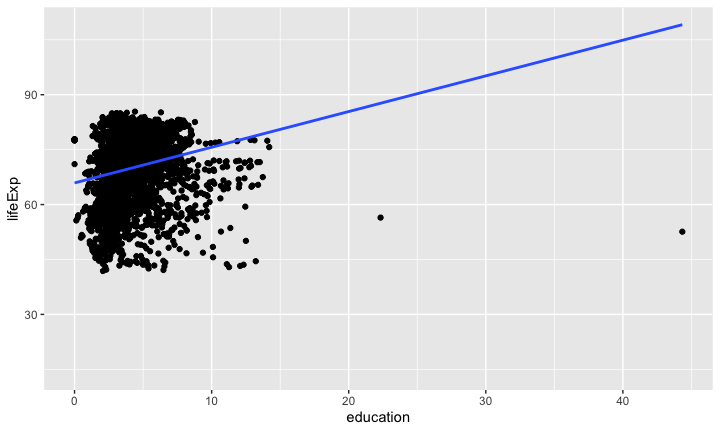
\includegraphics{eda5_files/figure-latex/unnamed-chunk-47-1.pdf}

\begin{Shaded}
\begin{Highlighting}[]
\NormalTok{wdi\_world }\SpecialCharTok{\%\textgreater{}\%} \FunctionTok{filter}\NormalTok{(income }\SpecialCharTok{!=} \StringTok{"Aggregates"}\NormalTok{) }\SpecialCharTok{\%\textgreater{}\%} \FunctionTok{drop\_na}\NormalTok{(education, lifeExp) }\SpecialCharTok{\%\textgreater{}\%} \FunctionTok{ggplot}\NormalTok{(}\FunctionTok{aes}\NormalTok{(education, lifeExp)) }\SpecialCharTok{+} \FunctionTok{geom\_point}\NormalTok{() }\SpecialCharTok{+} \FunctionTok{geom\_smooth}\NormalTok{(}\AttributeTok{formula =}\NormalTok{ y }\SpecialCharTok{\textasciitilde{}}\NormalTok{ x, }\AttributeTok{method =} \StringTok{"lm"}\NormalTok{, }\AttributeTok{se=}\ConstantTok{FALSE}\NormalTok{)}
\end{Highlighting}
\end{Shaded}

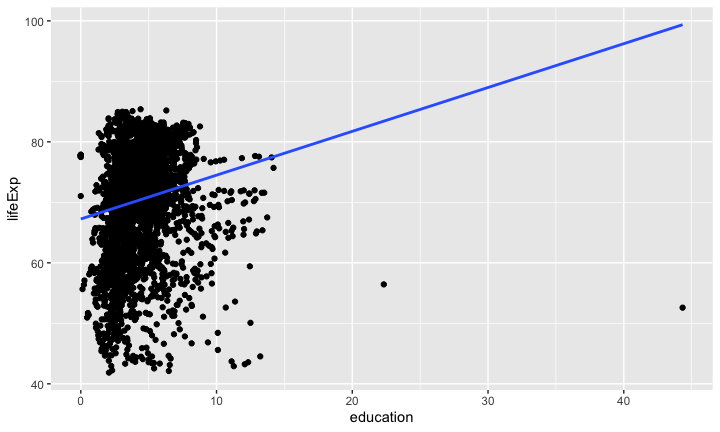
\includegraphics{eda5_files/figure-latex/unnamed-chunk-48-1.pdf}

\begin{Shaded}
\begin{Highlighting}[]
\NormalTok{wdi\_world\_el }\OtherTok{\textless{}{-}}\NormalTok{ wdi\_world }\SpecialCharTok{\%\textgreater{}\%} \FunctionTok{select}\NormalTok{(country, year, education, lifeExp, gdpPcap, pop, research, military, region, income) }\SpecialCharTok{\%\textgreater{}\%} \FunctionTok{filter}\NormalTok{(income }\SpecialCharTok{!=} \StringTok{"Aggregates"}\NormalTok{) }\SpecialCharTok{\%\textgreater{}\%} \FunctionTok{drop\_na}\NormalTok{(education, lifeExp)}
\end{Highlighting}
\end{Shaded}

\begin{Shaded}
\begin{Highlighting}[]
\NormalTok{wdi\_world\_el }\SpecialCharTok{\%\textgreater{}\%} \FunctionTok{ggplot}\NormalTok{(}\FunctionTok{aes}\NormalTok{(education)) }\SpecialCharTok{+} \FunctionTok{geom\_histogram}\NormalTok{()}
\end{Highlighting}
\end{Shaded}

\begin{verbatim}
## `stat_bin()` using `bins = 30`. Pick better value with `binwidth`.
\end{verbatim}

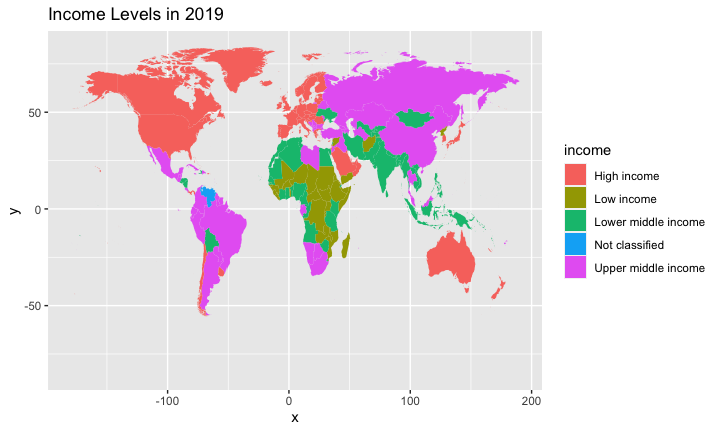
\includegraphics{eda5_files/figure-latex/unnamed-chunk-50-1.pdf}

\begin{Shaded}
\begin{Highlighting}[]
\NormalTok{wdi\_world\_el }\SpecialCharTok{\%\textgreater{}\%} \FunctionTok{filter}\NormalTok{(year}\SpecialCharTok{==}\DecValTok{2020}\NormalTok{) }\SpecialCharTok{\%\textgreater{}\%} \FunctionTok{ggplot}\NormalTok{(}\FunctionTok{aes}\NormalTok{(}\AttributeTok{x =}\NormalTok{ income, }\AttributeTok{y =}\NormalTok{ education, }\AttributeTok{fill =}\NormalTok{ income)) }\SpecialCharTok{+} \FunctionTok{geom\_boxplot}\NormalTok{()}
\end{Highlighting}
\end{Shaded}

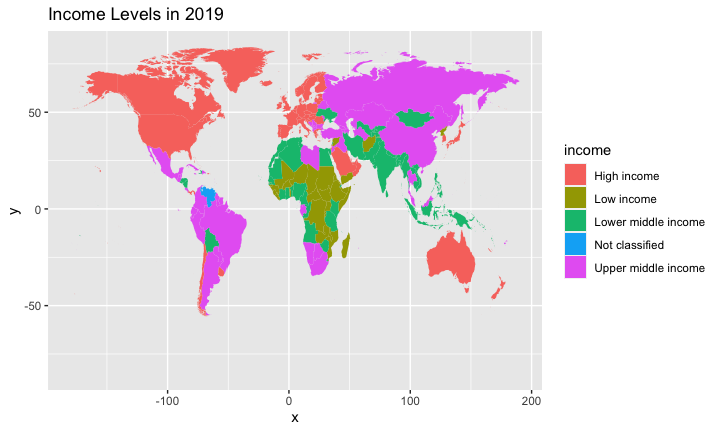
\includegraphics{eda5_files/figure-latex/unnamed-chunk-51-1.pdf}

\begin{Shaded}
\begin{Highlighting}[]
\NormalTok{wdi\_world\_el }\SpecialCharTok{\%\textgreater{}\%} \FunctionTok{filter}\NormalTok{(year}\SpecialCharTok{==}\DecValTok{2020}\NormalTok{) }\SpecialCharTok{\%\textgreater{}\%} \FunctionTok{arrange}\NormalTok{(}\FunctionTok{desc}\NormalTok{(education))}
\end{Highlighting}
\end{Shaded}

\begin{verbatim}
## # A tibble: 152 x 10
##    country     year educa~1 lifeExp gdpPcap    pop resea~2 milit~3 region income
##    <chr>      <dbl>   <dbl>   <dbl>   <dbl>  <dbl>   <dbl>   <dbl> <chr>  <chr> 
##  1 Solomon I~  2020   12.8     70.2   2080. 6.91e5  NA      NA     East ~ Lower~
##  2 Bolivia     2020    9.84    64.5   2920. 1.19e7  NA       1.32  Latin~ Lower~
##  3 Namibia     2020    9.45    62.8   4155. 2.49e6  NA       3.23  Sub-S~ Upper~
##  4 Sierra Le~  2020    8.81    59.8    604. 8.23e6  NA       0.547 Sub-S~ Low i~
##  5 Botswana    2020    8.74    65.6   5811. 2.55e6  NA       3.20  Sub-S~ Upper~
##  6 Saudi Ara~  2020    7.81    76.2  18086. 3.60e7   0.522   9.22  Middl~ High ~
##  7 Iceland     2020    7.72    83.1  52984. 3.66e5   2.47   NA     Europ~ High ~
##  8 Lesotho     2020    7.67    54.7    972. 2.25e6  NA       1.62  Sub-S~ Lower~
##  9 Cabo Verde  2020    7.58    74.8   2801. 5.83e5  NA       0.590 Sub-S~ Lower~
## 10 Belize      2020    7.53    72.9   5040. 3.95e5  NA       1.72  Latin~ Upper~
## # ... with 142 more rows, and abbreviated variable names 1: education,
## #   2: research, 3: military
\end{verbatim}

\begin{Shaded}
\begin{Highlighting}[]
\NormalTok{wdi\_world\_el }\SpecialCharTok{\%\textgreater{}\%} \FunctionTok{filter}\NormalTok{(year}\SpecialCharTok{==}\DecValTok{2020}\NormalTok{) }\SpecialCharTok{\%\textgreater{}\%} \FunctionTok{arrange}\NormalTok{(}\FunctionTok{desc}\NormalTok{(education))}
\end{Highlighting}
\end{Shaded}

\begin{verbatim}
## # A tibble: 152 x 10
##    country     year educa~1 lifeExp gdpPcap    pop resea~2 milit~3 region income
##    <chr>      <dbl>   <dbl>   <dbl>   <dbl>  <dbl>   <dbl>   <dbl> <chr>  <chr> 
##  1 Solomon I~  2020   12.8     70.2   2080. 6.91e5  NA      NA     East ~ Lower~
##  2 Bolivia     2020    9.84    64.5   2920. 1.19e7  NA       1.32  Latin~ Lower~
##  3 Namibia     2020    9.45    62.8   4155. 2.49e6  NA       3.23  Sub-S~ Upper~
##  4 Sierra Le~  2020    8.81    59.8    604. 8.23e6  NA       0.547 Sub-S~ Low i~
##  5 Botswana    2020    8.74    65.6   5811. 2.55e6  NA       3.20  Sub-S~ Upper~
##  6 Saudi Ara~  2020    7.81    76.2  18086. 3.60e7   0.522   9.22  Middl~ High ~
##  7 Iceland     2020    7.72    83.1  52984. 3.66e5   2.47   NA     Europ~ High ~
##  8 Lesotho     2020    7.67    54.7    972. 2.25e6  NA       1.62  Sub-S~ Lower~
##  9 Cabo Verde  2020    7.58    74.8   2801. 5.83e5  NA       0.590 Sub-S~ Lower~
## 10 Belize      2020    7.53    72.9   5040. 3.95e5  NA       1.72  Latin~ Upper~
## # ... with 142 more rows, and abbreviated variable names 1: education,
## #   2: research, 3: military
\end{verbatim}

\begin{Shaded}
\begin{Highlighting}[]
\NormalTok{wdi\_world\_el }\SpecialCharTok{\%\textgreater{}\%} \FunctionTok{filter}\NormalTok{(year}\SpecialCharTok{==}\DecValTok{2020}\NormalTok{) }\SpecialCharTok{\%\textgreater{}\%} \FunctionTok{lm}\NormalTok{(gdpPcap }\SpecialCharTok{\textasciitilde{}}\NormalTok{ education, .)}
\end{Highlighting}
\end{Shaded}

\begin{verbatim}
## 
## Call:
## lm(formula = gdpPcap ~ education, data = .)
## 
## Coefficients:
## (Intercept)    education  
##        9158         1285
\end{verbatim}

\begin{Shaded}
\begin{Highlighting}[]
\NormalTok{wdi\_world\_el }\SpecialCharTok{\%\textgreater{}\%} \FunctionTok{filter}\NormalTok{(year}\SpecialCharTok{==}\DecValTok{2020}\NormalTok{) }\SpecialCharTok{\%\textgreater{}\%} \FunctionTok{lm}\NormalTok{(gdpPcap }\SpecialCharTok{\textasciitilde{}}\NormalTok{ education, .) }\SpecialCharTok{\%\textgreater{}\%} \FunctionTok{glance}\NormalTok{()}
\end{Highlighting}
\end{Shaded}

\begin{verbatim}
## # A tibble: 1 x 12
##   r.squared adj.r.squa~1  sigma stati~2 p.value    df logLik   AIC   BIC devia~3
##       <dbl>        <dbl>  <dbl>   <dbl>   <dbl> <dbl>  <dbl> <dbl> <dbl>   <dbl>
## 1    0.0131      0.00650 20523.    1.98   0.161     1 -1713. 3431. 3440. 6.28e10
## # ... with 2 more variables: df.residual <int>, nobs <int>, and abbreviated
## #   variable names 1: adj.r.squared, 2: statistic, 3: deviance
\end{verbatim}

\begin{Shaded}
\begin{Highlighting}[]
\NormalTok{wdi\_world\_el }\SpecialCharTok{\%\textgreater{}\%} \FunctionTok{lm}\NormalTok{(lifeExp }\SpecialCharTok{\textasciitilde{}}\NormalTok{ education }\SpecialCharTok{+}\NormalTok{ research }\SpecialCharTok{+}\NormalTok{ military, .) }\SpecialCharTok{\%\textgreater{}\%} \FunctionTok{glance}\NormalTok{()}
\end{Highlighting}
\end{Shaded}

\begin{verbatim}
## # A tibble: 1 x 12
##   r.squared adj.r.squ~1 sigma stati~2   p.value    df logLik   AIC   BIC devia~3
##       <dbl>       <dbl> <dbl>   <dbl>     <dbl> <dbl>  <dbl> <dbl> <dbl>   <dbl>
## 1     0.346       0.345  5.25    270. 2.05e-140     3 -4711. 9432. 9458.  42036.
## # ... with 2 more variables: df.residual <int>, nobs <int>, and abbreviated
## #   variable names 1: adj.r.squared, 2: statistic, 3: deviance
\end{verbatim}

\begin{Shaded}
\begin{Highlighting}[]
\NormalTok{wdi\_world\_el }\SpecialCharTok{\%\textgreater{}\%} \FunctionTok{lm}\NormalTok{(lifeExp }\SpecialCharTok{\textasciitilde{}}\NormalTok{ education }\SpecialCharTok{+}\NormalTok{ research }\SpecialCharTok{+}\NormalTok{ military, .) }\SpecialCharTok{\%\textgreater{}\%} \FunctionTok{tidy}\NormalTok{()}
\end{Highlighting}
\end{Shaded}

\begin{verbatim}
## # A tibble: 4 x 5
##   term        estimate std.error statistic   p.value
##   <chr>          <dbl>     <dbl>     <dbl>     <dbl>
## 1 (Intercept)  70.2       0.489    144.    0        
## 2 education     0.0771    0.0966     0.798 4.25e-  1
## 3 research      3.84      0.145     26.4   6.95e-127
## 4 military     -0.0682    0.102     -0.667 5.05e-  1
\end{verbatim}

\[lifeExp \sim 70.22 + 0.08\cdot education + 3.84 \cdot research - 0.07 \cdot military\]

\begin{Shaded}
\begin{Highlighting}[]
\NormalTok{wdi\_world\_el }\SpecialCharTok{\%\textgreater{}\%} \FunctionTok{lm}\NormalTok{(gdpPcap }\SpecialCharTok{\textasciitilde{}}\NormalTok{ education }\SpecialCharTok{+}\NormalTok{ research }\SpecialCharTok{+}\NormalTok{ military, .) }\SpecialCharTok{\%\textgreater{}\%} \FunctionTok{tidy}\NormalTok{()}
\end{Highlighting}
\end{Shaded}

\begin{verbatim}
## # A tibble: 4 x 5
##   term        estimate std.error statistic   p.value
##   <chr>          <dbl>     <dbl>     <dbl>     <dbl>
## 1 (Intercept)    1077.     1308.     0.823 4.11e-  1
## 2 education      1324.      258.     5.12  3.41e-  7
## 3 research      12792.      389.    32.9   1.07e-179
## 4 military       -967.      273.    -3.54  4.08e-  4
\end{verbatim}

\begin{Shaded}
\begin{Highlighting}[]
\NormalTok{wdi\_world\_el }\SpecialCharTok{\%\textgreater{}\%} \FunctionTok{lm}\NormalTok{(gdpPcap }\SpecialCharTok{\textasciitilde{}}\NormalTok{ education }\SpecialCharTok{+}\NormalTok{ research }\SpecialCharTok{+}\NormalTok{ military, .) }\SpecialCharTok{\%\textgreater{}\%} \FunctionTok{glance}\NormalTok{()}
\end{Highlighting}
\end{Shaded}

\begin{verbatim}
## # A tibble: 1 x 12
##   r.squared adj.r~1  sigma stati~2   p.value    df  logLik    AIC    BIC devia~3
##       <dbl>   <dbl>  <dbl>   <dbl>     <dbl> <dbl>   <dbl>  <dbl>  <dbl>   <dbl>
## 1     0.478   0.477 14013.    466. 9.65e-215     3 -16766. 33542. 33569. 2.99e11
## # ... with 2 more variables: df.residual <int>, nobs <int>, and abbreviated
## #   variable names 1: adj.r.squared, 2: statistic, 3: deviance
\end{verbatim}

\[gdpPcap \sim 1077 + 1024\cdot education + 12792 \cdot research - 967 \cdot military\]

\begin{Shaded}
\begin{Highlighting}[]
\NormalTok{mod\_r }\OtherTok{\textless{}{-}} \FunctionTok{lm}\NormalTok{(lifeExp }\SpecialCharTok{\textasciitilde{}}\NormalTok{ research, wdi\_world); mod\_e}
\end{Highlighting}
\end{Shaded}

\begin{verbatim}
## 
## Call:
## lm(formula = lifeExp ~ education, data = wdi_world)
## 
## Coefficients:
## (Intercept)    education  
##     65.9047       0.9748
\end{verbatim}

\hypertarget{model-and-linear-regression-quick-reference}{%
\subsubsection{model and Linear Regression Quick
Reference}\label{model-and-linear-regression-quick-reference}}

\begin{itemize}
\tightlist
\item
  R4DS: Model basics

  \begin{itemize}
  \tightlist
  \item
    \url{https://r4ds.had.co.nz/model-basics.html}
  \end{itemize}
\end{itemize}

For explanation of other indices, please see.

\begin{itemize}
\tightlist
\item
  r-statistics.co by Selva Prabhakaran:

  \begin{itemize}
  \tightlist
  \item
    \url{http://r-statistics.co/Linear-Regression.html}
  \end{itemize}
\end{itemize}

\begin{center}\rule{0.5\linewidth}{0.5pt}\end{center}

\hypertarget{roudups}{%
\subsection{Roudups}\label{roudups}}

\begin{center}\rule{0.5\linewidth}{0.5pt}\end{center}

\hypertarget{r-markdown-revisited}{%
\subsubsection{R Markdown Revisited}\label{r-markdown-revisited}}

Presentation: Submit an R Notebook (with codes used in the
presentation), and PowerPoint file or other files used for your
presentation, if any. If you use R Notebook for your presentation, you
do not need to submit extra files.

Final Paper: Submit an R Notebook (with codes as a work file), and a PDF
(rendered directly from an R Notebook, or created from Word) - Maximum
pages of PDF is eight.

Format of Presentation - R Notebook is fine and slide presentation in
various format is also fine

\begin{center}\rule{0.5\linewidth}{0.5pt}\end{center}

\hypertarget{literate-programming-and-reproducible-research}{%
\paragraph{Literate Programming and Reproducible
Research}\label{literate-programming-and-reproducible-research}}

Importing Data:

\begin{enumerate}
\def\labelenumi{\arabic{enumi}.}
\tightlist
\item
  Read a csv file: \texttt{read\_csv("data/file\_name.csv")}
\item
  Download and import using a url of a csv file: \texttt{read\_csv(url)}
\item
  Read an Excel file:
  \texttt{readxl::read\_excel("data/excel\_file\_name.xlsx")}
\item
  Read from the clipboard: \texttt{read\_delim(clipboard())}
\end{enumerate}

\begin{itemize}
\tightlist
\item
  zip file:

  \begin{itemize}
  \item
    copy the url
  \item
    wir1to10 \textless-
    ``\url{https://wir2022.wid.world/www-site/uploads/2022/03/WIR2022TablesFigures-Chapter.zip}''
  \item
    download.file(wir1to10, destfile = ``data/wir1to10.zip'')
  \item
    unzip(``data/wir1to10.zip'', exdir = ``data'')
  \item
    list.files(``data/WIR2022TablesFigures-Chapter'')
  \item
    excel\_sheets(``data/WIR2022TablesFigures-Chapter/WIR2022TablesFigures-Chapter1.xlsx'')
  \item
    df \textless- read\_delim(clipboard()); df
  \item
    Not reproducible unless clearly explained.
  \end{itemize}
\end{itemize}

\begin{center}\rule{0.5\linewidth}{0.5pt}\end{center}

\hypertarget{code-chunk-options}{%
\paragraph{Code Chunk Options}\label{code-chunk-options}}

\url{https://yihui.org/knitr/options/}

\begin{itemize}
\item
  Chunk Name
\item
  Output: use document default

  \begin{itemize}
  \tightlist
  \item
    Show code and output: echo=TRUE, eval=TRUE - Default
  \item
    Show output only: echo=FALSE
  \item
    Show nothing (run code): include=FALSE
  \item
    Show nothing (don't run code): include=FALSE, eval=FALSE
  \end{itemize}
\item
  Show message: message=TRUE, FALSE
\item
  Show warning: warning=TRUE, FALSE
\item
  Use Paged Tables: paged.print=TRUE, FALSE
\item
  Use custom figure size: width and height in inch.
\item
  You can use Hide Code and Show Code option on the rendered Notebook
  file.
\end{itemize}

\begin{center}\rule{0.5\linewidth}{0.5pt}\end{center}

\hypertarget{presentation-and-paper}{%
\paragraph{Presentation and Paper}\label{presentation-and-paper}}

\begin{enumerate}
\def\labelenumi{\arabic{enumi}.}
\item
  Data Source
\item
  Variables
\item
  Problems
\item
  Visualization
\item
  Model
\item
  Conclusions and Further Research

  WDI, WIR, etc
\end{enumerate}

\begin{center}\rule{0.5\linewidth}{0.5pt}\end{center}

\hypertarget{word}{%
\paragraph{Word}\label{word}}

Custom Word templates:
\url{https://bookdown.org/yihui/rmarkdown-cookbook/word-template.html}

You can apply the styles defined in a Word template document to new Word
documents generated from R Markdown. Such a template document is also
called a ``style reference document.'' The key is that you have to
create this template document from Pandoc first, and change the style
definitions in it later. Then pass the path of this template to the
reference\_docx option of word\_document

\begin{verbatim}
---
 word_document:
    reference_docx: "template.docx"
---
\end{verbatim}

\begin{center}\rule{0.5\linewidth}{0.5pt}\end{center}

\hypertarget{powerpoint}{%
\paragraph{PowerPoint}\label{powerpoint}}

PowerPoint presentation:
\url{https://bookdown.org/yihui/rmarkdown/powerpoint-presentation.html}

Custom templates:
\url{https://bookdown.org/yihui/rmarkdown/powerpoint-presentation.html\#ppt-templates}

\begin{verbatim}
---
  powerpoint_presentation:
    reference_doc: my-styles.pptx
---
\end{verbatim}

\url{https://support.microsoft.com/en-us/office/create-and-save-a-powerpoint-template-ee4429ad-2a74-4100-82f7-50f8169c8aca}

YouTube: How To Create A PowerPoint Template

\begin{center}\rule{0.5\linewidth}{0.5pt}\end{center}

\hypertarget{the-week-six-assignment---assignment-five-in-moodle}{%
\subsection{The Week Six Assignment - Assignment Five (in
Moodle)}\label{the-week-six-assignment---assignment-five-in-moodle}}

\begin{itemize}
\tightlist
\item
  Create an R Notebook of a Data Analysis containing the following and
  submit the rendered HTML file (eg. \texttt{a5\_123456.nb.html} by
  replacing 123456 with your ID), and a PDF (or MS Word File).

  \begin{enumerate}
  \def\labelenumi{\arabic{enumi}.}
  \tightlist
  \item
    create an R Notebook using the R Notebook Template in Moodle, save
    as \texttt{a3\_123456.Rmd},
  \item
    write your name and ID and the contents,
  \item
    run each code block,
  \item
    preview to create \texttt{a5\_123456.nb.html},
  \item
    render (or knit) PDF, or Word (and then PDF)
  \item
    submit \texttt{a5\_123456.nb.html} and PDF (or Word) to Moodle.
  \end{enumerate}
\end{itemize}

\begin{enumerate}
\def\labelenumi{\arabic{enumi}.}
\item
  Choose a data with at least two numerical variables. One of them can
  be the year.

  \begin{itemize}
  \tightlist
  \item
    Information of the data
  \item
    Explain why you chose the data
  \item
    List questions you want to study
  \end{itemize}
\end{enumerate}

\begin{center}\rule{0.5\linewidth}{0.5pt}\end{center}

\begin{enumerate}
\def\labelenumi{\arabic{enumi}.}
\setcounter{enumi}{1}
\item
  Explore the data using visualization using \texttt{ggplot2}

  \begin{itemize}
  \tightlist
  \item
    Create various charts, and write observed comments
  \item
    Apply a (linear regression) model, and draw a regression line to at
    least one chart, and write your conclusion based on the model using
    the slope value and R squared (and/or adjusted R squared).
  \end{itemize}
\item
  Observations based on your exploratory data analysis, and difficulties
  and questions encountered if any.
\end{enumerate}

\textbf{Due:} 2023-01-30 23:59:00. Submit your R Notebook file, and a
PDF file (or an MS Word file) in Moodle (The Fifth Assignment). Due on
Monday!

\begin{center}\rule{0.5\linewidth}{0.5pt}\end{center}

\hypertarget{roundup}{%
\subsection{Roundup}\label{roundup}}

\hypertarget{history-of-regression-analysis-slope-0.4465}{%
\subsubsection{History of Regression Analysis: slope =
0.4465}\label{history-of-regression-analysis-slope-0.4465}}

\begin{quote}
The heights of descendants of tall ancestors tend to regress down
towards a normal average
\end{quote}

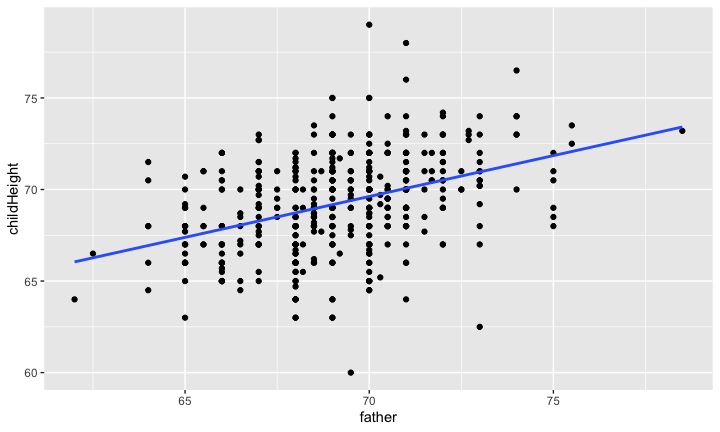
\includegraphics{eda5_files/figure-latex/unnamed-chunk-61-1.pdf}

\begin{Shaded}
\begin{Highlighting}[]
\NormalTok{gf }\SpecialCharTok{\%\textgreater{}\%} \FunctionTok{filter}\NormalTok{(gender }\SpecialCharTok{==} \StringTok{"male"}\NormalTok{) }\SpecialCharTok{\%\textgreater{}\%} \FunctionTok{lm}\NormalTok{(childHeight }\SpecialCharTok{\textasciitilde{}}\NormalTok{ father, .)}
\end{Highlighting}
\end{Shaded}

\begin{verbatim}
## 
## Call:
## lm(formula = childHeight ~ father, data = .)
## 
## Coefficients:
## (Intercept)       father  
##     38.3626       0.4465
\end{verbatim}

\begin{center}\rule{0.5\linewidth}{0.5pt}\end{center}

\hypertarget{anna-karenina-principle}{%
\subsubsection{Anna Karenina Principle}\label{anna-karenina-principle}}

\begin{quote}
``Tidy data sets are all alike; but every messy data set is messy in its
own way.'' --- Hadley Wickham
\end{quote}

\begin{quote}
``all happy families are all alike; each unhappy family is unhappy in
its own way'' - Tolstoy's Anna Karenina
\end{quote}

The Anna Karenina principle states that a deficiency in any one of a
number of factors dooms an endeavor to failure. Consequently, a
successful endeavor (subject to this principle) is one for which every
possible deficiency has been avoided. (Wikipedia)

Please look at the outliers carefully.

\end{document}
